\documentclass{book}
\usepackage[top=20mm,bottom=20mm,left=20mm,right=20mm,a4paper]{geometry}
\usepackage{microtype,soul,filecontents}
\usepackage{pgf}
\usepackage{lettrine,caption,multicol}
\usepackage{xcolor}
\usepackage{lipsum,soul}
\usepackage{palatino}
\usepackage{calligra}
\usepackage[T1]{fontenc}
\makeatletter
\usepackage[listings,theorems]{tcolorbox}
%\usepackage[charter]{mathdesign}
% \def\rmdefault{bch} % not scaled
% \def\ttdefault{blg}
\usepackage{xcolor,filecontents,ragged2e}
\definecolor{theblue} {rgb}{0.02,0.04,0.48}
\definecolor{thered}  {rgb}{0.65,0.04,0.07}
\definecolor{thegreen}{rgb}{0.06,0.44,0.08}
\definecolor{thegrey} {gray}{0.5}
\definecolor{theshade}{gray}{0.94}
\definecolor{theframe}{gray}{0.75}
\newcommand\lorem{Fusce adipiscing justo nec ante. Nullam in enim.
 Pellentesque felis orci, sagittis ac, malesuada et, facilisis in,
 ligula. Nunc non magna sit amet mi aliquam dictum. In mi. Curabitur
 sollicitudin justo sed quam et quadd. \par}

\lstloadlanguages{[LaTeX]TeX, [primitive]TeX}

% Emphasis
\newcommand\emphasis[2][thered]{\lstset{emph={newcommand,def,gdef,#2},
   emphstyle={\ttfamily\textcolor{#1}}}}%

\lstset{language={[LaTeX]TeX},
      escapeinside={{(*@}{@*)}}, 
       numbers=left, gobble=0,
       stepnumber=1,numbersep=5pt, 
       numberstyle={\footnotesize\color{gray}},firstnumber=last,
       breaklines=true,
       framesep=5pt,
       basicstyle=\small\ttfamily,
       showstringspaces=false,
     % keywordstyle=\ttfamily\textcolor{thegreen},
      stringstyle=\color{orange},
      commentstyle=\color{black},
      rulecolor=\color{theshade},
      breakatwhitespace=true,
     showspaces=false,  % shows spacing symbol
      xleftmargin=0pt,
      xrightmargin=5pt,
      aboveskip=3pt plus1pt minus1pt, % compact the code looks ugly in type
      belowskip=7pt plus1pt minus1pt,  % user responsible to insert any skips
      backgroundcolor=\color{theshade}
}

\begin{filecontents*}{chapterx.sty}
\ProvidesPackage{chapters}[2012/04/07 v0.1 Typesetting chapters]
\newcommand\HUGE{\@setfontsize\Huge{38}{47}}
\newcommand\HHUGE{\@setfontsize\HHUGE{58}{67}}


\newenvironment{summary}
               {\list{}{\listparindent0pt %
                        \itemindent\listparindent
                        \leftmargin0pt
                        \rightmargin\leftmargin
                        \parsep\z@ \@plus\p@}%
                \item\relax\itshape}
               {\endlist}

% helper macros
\gdef\thinrule{\rule{\textwidth}{0.4pt}}
\gdef\mediumrule{\rule{\textwidth}{0.8pt}}
%% broad positions
\newif\if@left
\newif\if@right
\newif\if@center
\@leftfalse
\@rightfalse
\@centerfalse
% newifs for number position
\newif\if@lefttitle
\newif\if@righttitle
\newif\if@leftname
\newif\if@rightname
\newif\if@chapterspaceout\@chapterspaceoutfalse
\newif\if@titlespaceout\@chapterspaceoutfalse

%\section{Libraries} 

\def\cx@optionlist{}


\def\cx@optionlist{}

\def\cxuselibrary#1{\cxset{library/.cd,#1}}
%
% The library is added by inputting the file and setting the path accordingly.
\def\cx@add@library#1#2{%
  \cxset{library/#1/.code={\@ifundefined{cxlibrary@#1@loaded}{\input #2}{}}}%
  \DeclareOption{#1}{\edef\cx@optionlist{\cx@optionlist,#1}}%
}

\def\thickrule{\leavevmode \leaders \hrule height 3pt \hfill \kern \z@}


% Define a family for chapter styling keys
\pgfkeys{/chapter/.is family}



\def\cxset{\pgfqkeys{/chapter}} %Notice this is pgf q keys
% spent half the evening to debug it;)Aarg!!!
% We define keys for all major components
\cxset{%
  name/.code={\gdef\chaptername{#1}},
  color/.store in=\color@cx,
  color/.default=black,
  chapter font-family/.store in=\chapterfontfamily@cx,
  chapter font-weight/.store in=\chapterfontweight@cx,
  chapter font-size/.store in=\chapterfontsize@cx,
  chapter color/.store in=\chaptercolor@cx,
  chapter before/.store in=\chapterbefore@cx,
  chapter after/.store in=\chapterafter@cx,
  chapter spaceout/.is choice,
  chapter spaceout/soul/.code={\@chapterspaceouttrue},
  chapter spaceout/none/.code={\@chapterspaceoutfalse},
  % title keys
  title font-family/.store in=\titlefontfamily@cx,
  title font-family/.default=\rmfamily,
  title font-weight/.store in=\titlefontweight@cx,
  title font-size/.store in=\titlefontsize@cx,
  title font-color/.store in=\titlefontcolor@cx,
  title spaceout/.is choice,
  title spaceout/soul/.code={\@titlespaceouttrue},
  title spaceout/none/.code={\@titlespaceoutfalse},
  title font/.style={title font-family=#1},
  title before/.store in=\titlebefore@cx,
  title after/.store in=\titleafter@cx,
  title beforeskip/.store in=\titlebeforeskip@cx,
  title afterskip/.store in=\titleafterskip@cx,
  position/.is choice,
  position/left/.code={\@lefttrue},
  position/right/.code={\@righttrue},
  position/center/.code={\@centertrue},
% numbering options that are required
  numbering/.is choice,
% better to rename thechapter?
  numbering/roman/.code={\gdef\thechapter{\@roman\c@chapter}},
  numbering/Roman/.code={\gdef\thechapter{\@Roman\c@chapter}},
  numbering/arabic/.code={\gdef\thechapter{\@arabic\c@chapter}},
  numbering/none/.code={\gdef\thechapter{}},
  number dot/.store in=\numberpunctuation@cx,
  number position/.is choice,
  number position/leftname/.code={\@leftnametrue\@rightnamefalse},
  number position/rightname/.code={\@rightnametrue\@leftnamefalse},
  number position/absolute/.code={},
  number position/righttitle/.code={\@righttitletrue},
  number position/lefttitle/.code={\@lefttitletrue},
  number after/.store in=\numberafter@cx,
  number before/.store in=\numberbefore@cx,
  number color/.store in=\numbercolor@cx,
  number font-size/.store in=\numberfontsize@cx,
  number font-family/.store in=\numberfontfamily@cx,
  number font-weight/.store in=\numberfontweight@cx,
% headers and footers
  header style/.store in=\headerstyle@cx,
% general draft rules
  rule /.is choice,
  rule on/.code={\gdef\rulewidth@cx{0.4pt}},
  rule off/.code={\gdef\rulewidth@cx{0pt}},
}

\cxset{%
  color=blue,
  position=center,
  name=chapteris,
  title font-family=\rmfamily,
  title font-weight=\bfseries,
  title font-size=\Huge,
  title font-color=\color{olive},
  numbering=arabic,
  number dot=,
  chapter font-family=\sffamily,
  chapter font-weight=\bfseries,
  chapter font-size=\Large,
  chapter color=gray,
  chapter before={\leavevmode\par\hfill},%need to correct for 0pt
  chapter after=\hfill\hfill,
  number position=rightname,
  number color=\color{gray},
  number after=\hspace{20pt},
  number before=\hspace*{20pt},
  number font-size=\huge,
  number font-family=\sffamily,
  number font-weight=\bfseries,
  number before=,
  number after=,
  title before=,
  title after=,
  title afterskip={\vskip50pt},
  title beforeskip={\vskip10pt},
  header style=plain,
}

\gdef\setdefaults{%
\cxset{%
name=CHAPTER,
title font-family=\rmfamily,
title font-weight=\bfseries,
title font-size=\Huge,
title font-color=\color{purple},
numbering=arabic,
number dot=,
number before=,
number after=,
chapter font-family=\sffamily,
chapter font-weight=\bfseries,
chapter font-size=\large,
chapter spaceout=soul,
chapter color=gray,
chapter before={},%need to correct for 0pt
chapter after=,
number position=rightname,
number color=\color{gray},
number after=\hspace{20pt},
number before=\space,
number font-size=\large,
number font-family=\sffamily,
number font-weight=\bfseries,
title before=,
title after=,
title afterskip={\vskip24pt},
title beforeskip={\vskip10pt},
title font=\rmfamily,
header style=plain,
}
}

% The |\@makechapterhead| is used by LaTeX to typeset the
% Chapter heading. This is a rewrite in order to make it
% more flexible and use the keys.

\renewcommand\@makechapterhead[2][]{%
% macro for typesetting the chapter number
  \def\printnumber{%
    \numberbefore@cx
      {%
      \numbercolor@cx
      \numberfontsize@cx
      \numberfontfamily@cx
      \numberfontweight@cx
      \thechapter
      \numberpunctuation@cx
      }
      \numberafter@cx
  }%
% macro for typesetting the chapter name
  \def\printchaptername{%
    {
    \chapterfontfamily@cx
    \chapterfontsize@cx
    \chapterfontweight@cx
    \color{\chaptercolor@cx}
% Check if the chapter name is spaced out and use the
% soul package. TODO add values for soul parameters
% as a style feature.
    \if@chapterspaceout 
     \expandafter\so\expandafter{\chaptername}
    \else
      \@chapapp\space
    \fi
    }%
  }%
% set all keys
    {%
    \parindent0pt 
    \normalfont%
    \ifnum \c@secnumdepth>\m@ne%
      \if@mainmatter%
 % we start displaying  the names and any preambles such 
 % as images
 % print chapter name
         \chapterbefore@cx%
         \if@leftname
            \printnumber
         \fi%
         \printchaptername
         \if@rightname
            \printnumber
         \fi%
         \chapterafter@cx  
      \fi%
    \fi%
     %chapter title
    \interlinepenalty\@M%
% if the number is before the title
% if the number prints together with the title they 
% are considered as one indivisible part.
     \titlebeforeskip@cx%
     \if@lefttitle%
       \beforenumber@cx%
       \counterdisplay\c@chapter\afternumber@cx%
     \fi
% Display title
      \titlefontfamily@cx
      \titlefontweight@cx
      \titlefontsize@cx
      \titlefontcolor@cx
      \selectfont
      \titlebefore@cx%
      \if@titlespaceout
         \so{#2}%
      \else
         #2
      \fi%
      \titleafter@cx
    \if@righttitle%
      \afternumber@cx
      \counterdisplay\c@chapter\afternumber@cx%
    \fi
    \par\nobreak%
% skip after title
    \titleafterskip@cx
% headers
    \thispagestyle{\headerstyle@cx}
}}


%% Special Chapter command
\newcommand\specialchapter@cx[2][]{%
\cxset{image/.store in=\image@cx,
       image caption/.store in=\caption@cx}
\cxset{#1}
\vbox to 0pt{\color{blue}\rule{\paperwidth}{0.4pt}\par\vskip-1.4pt
\rule{0.4pt}{\textheight}\rule{4cm}{0.4pt}}

\vbox to 0pt{\parbox[b]{4.7cm}{%
\raggedright

\leftskip1.5cm
\caption@cx\par
 \expandafter\rule{\rulewidth@cx}{5.8cm}
}\parbox[b]{0.5cm}{
\includegraphics[width=0.5cm,height=9.15cm]{./chapters/shadow}}\includegraphics{./chapters/\image@cx}\par}

\vspace{8.2cm}
\hspace*{-3.51cm}\hbox to 0pt{\hspace*{1.01cm}
\includegraphics[width=7.7cm,height=3.8cm]{./chapters/genetics-band}
\hspace*{-2.7cm}\sffamily\color{\numbercolor@cx}\HHUGE \raise30pt\hbox{4}%
\hspace{1.5cm}\raise0.5pt\hbox{
\includegraphics{./chapters/chapterconcept}
\includegraphics{./chapters/shadow2}}
}

%% Title name
\parbox[b]{0.45\textwidth}{%
  \titlefontsize@cx
  \titlefontweight@cx
  \titlefontfamily@cx
  \leftskip0.5em \color{\titlefontcolor@cx}
  #2
}
%% Concepts
}

\newenvironment{specialchapter}[2][]{%
  \if@openright\cleardoublepage\else\clearpage\fi
    \thispagestyle{plain}%
    \global\@topnum\z@
    \@afterindentfalse
    \specialchapter@cx[#1]{#2}
    \begin{minipage}{0.5\textwidth}%
    \vspace{0.5\baselineskip}
    \raggedright
}{\end{minipage}}
\end{filecontents*}

\usepackage{chapterx}
\usepackage{makeidx}
\makeindex
\author{Y Lazarides}
\title{\parindent0pt A New Approach in\\ Styling Chapters}
\begin{document}
\maketitle
\tableofcontents
\mainmatter
\setdefaults
\chapter{Introduction}
The aim of the package is to allow easy styling of chapter heads and extends these to include images and special effects, which are difficult to achieve using traditional methods. 

Abstracting the various designs is a non-trivial undertaking due to the hundreds of different possibilities.

\section{Background}

The \LaTeX2e\ method of constructing the layout for Chapters is complicated and spread all over the book.cls code. Although not very difficult to customize, customization is not user friendly. 

\begin{description}
\item [counters] Counters can be displayed or not. These are constructed using the normal LaTeX method.
   \begin{verbatim}
   \renewcommand \thechapter {\@arabic\c@chapter}
   \end{verbatim}

\item [name] Here we use the term \textit{name} to denote in english the word ``chapter''. This can be typeset differently, depending on the language. It depends on on redefining one macro.
   \begin{verbatim}
     \def\chaptername{Chapter}
   \end{verbatim}
\item [openright] The global option open right, triggers the typesetting of chapter on odd pages only. There are a  couple of layouts that must be typeset on an even pages.

\item [\string\chapter] The chapter command is the main author command and where all the branching starts.
    \begin{verbatim}
\newcommand\chapter{%
  \if@openright\cleardoublepage\else\clearpage\fi
    \thispagestyle{plain}%
    \global\@topnum\z@
    \@afterindentfalse
    \secdef\@chapter\@schapter}
    \end{verbatim}

One limitation for this command is that it always starts a chapter on a new page and the macro needs to be rewritten if for example a new chapter is allowed to start anywhere.

Consider options openright, openleft, continuous.

The pagestyle is also settled here.

secdef will define basic macros for chaapter and starred chapter. What it basically does... this will become unecessary as we are going to find out a bit later on, but first the @chapter.

\item [\string\@chapter] This is the basic routine
\begin{verbatim}
\def\@chapter[#1]#2{
  \ifnum \c@secnumdepth >\m@ne
    \if@mainmatter
      \refstepcounter{chapter}%
      \typeout{\@chapapp\space\thechapter.}%
      \addcontentsline{toc}{chapter}%
         {\protect\numberline{\thechapter}#1}%
      \else
         \addcontentsline{toc}{chapter}{#1}%
    \fi
  \else
    \addcontentsline{toc}{chapter}{#1}%
  \fi
  \chaptermark{#1}%
  \addtocontents{lof}{\protect\addvspace{10\p@}}%
  \addtocontents{lot}{\protect\addvspace{10\p@}}%
  \if@twocolumn
    \@topnewpage[\@makechapterhead{#2}]%
  \else
    \@makechapterhead{#2}%
    \@afterheading
  \fi}
\end{verbatim}
  The important branching command here is makechapterhead,   which is responsible for typesetting the layout.

\end{description}

\section{Counters}
\begin{verbatim}

\renewcommand \thepart {\@Roman\c@part}
\renewcommand \thechapter {\@arabic\c@chapter}
\end{verbatim}



\section{major components}

The major components of a chapter opening, is the chapter name, the number and the title. It can be enclosed in boxes rules or other decorative elements. 

One peculiarity is how to specify the position of the number.

leftofchaptername rightofchaptername ownline 

\subsection{algorithmic approach}

All major components are saved in boxes. then based on booleans or templets are inserted in right location. Similar to objects.

\clearpage
%% GENETICS
\cxset{
 name={CHAPTER CONCEPT},
 numbering=none,
 number font-size=,
 number font-family=,
 number font-weight=,
 number color=white,
 chapter color={black},
 chapter font-family=\sffamily,
 chapter font-size=\large,
 chapter font-weight=\bfseries,
 title font-family=\sffamily,
 title font-color=teal,
 rule off,
}


\begin{specialchapter}[
     image=chromosome,%genetics-dogs,
     image caption={Labrador retriever\\
         puppies expressing\\
         brown (chocolate),\\
         golden (yellow),\\
         and black\\
         coat colors,\\
         traits controlled\\
         by two gene pairs.}]%
{Extensions\\ of Mendelian\\ Genetics}
\begin{itemize}
\item While alleles are transmitted from parent to   offspring
according to Mendelian principles, they often do not
display the clear-cut dominant/recessive relationship
observed by Mendel.
\item In many cases, in a departure from Mendelian genetics,
two or more genes are known to influence the phenotype
of a single characteristic.
\item Still another exception to Mendelian inheritance occurs
when genes are located on the X chromosome, because one
of the sexes receives only one copy of that chromosome,
eliminating the possibility of heterozygosity.
\item Phenotypes are often the combined result of genetics and
the environment within which genes are expressed.
\item The result of the various exceptions to Mendelian principles
is the occurrence of phenotypic ratios that differ from those
produced by standard monohybrid, dihybrid, and trihybrid
crosses.
  \end{itemize}
\end{specialchapter}


%% EDDOUARD MANET
\cxset{manet/.style={
 name={},
 numbering=none,
 number font-size=,
 number font-family=,
 number font-weight=,
 number before={\vspace*{-2.5cm}},
 number dot={},
 number after={},
 number position=leftname,
 chapter font-family=,
 chapter font-weight=,
 chapter font-size=,
 chapter before={},
 chapter after={},
 chapter color={black!90},
 number color=\color{purple},
 title beforeskip={},
 title afterskip={},
 title before={\hskip-2.3cm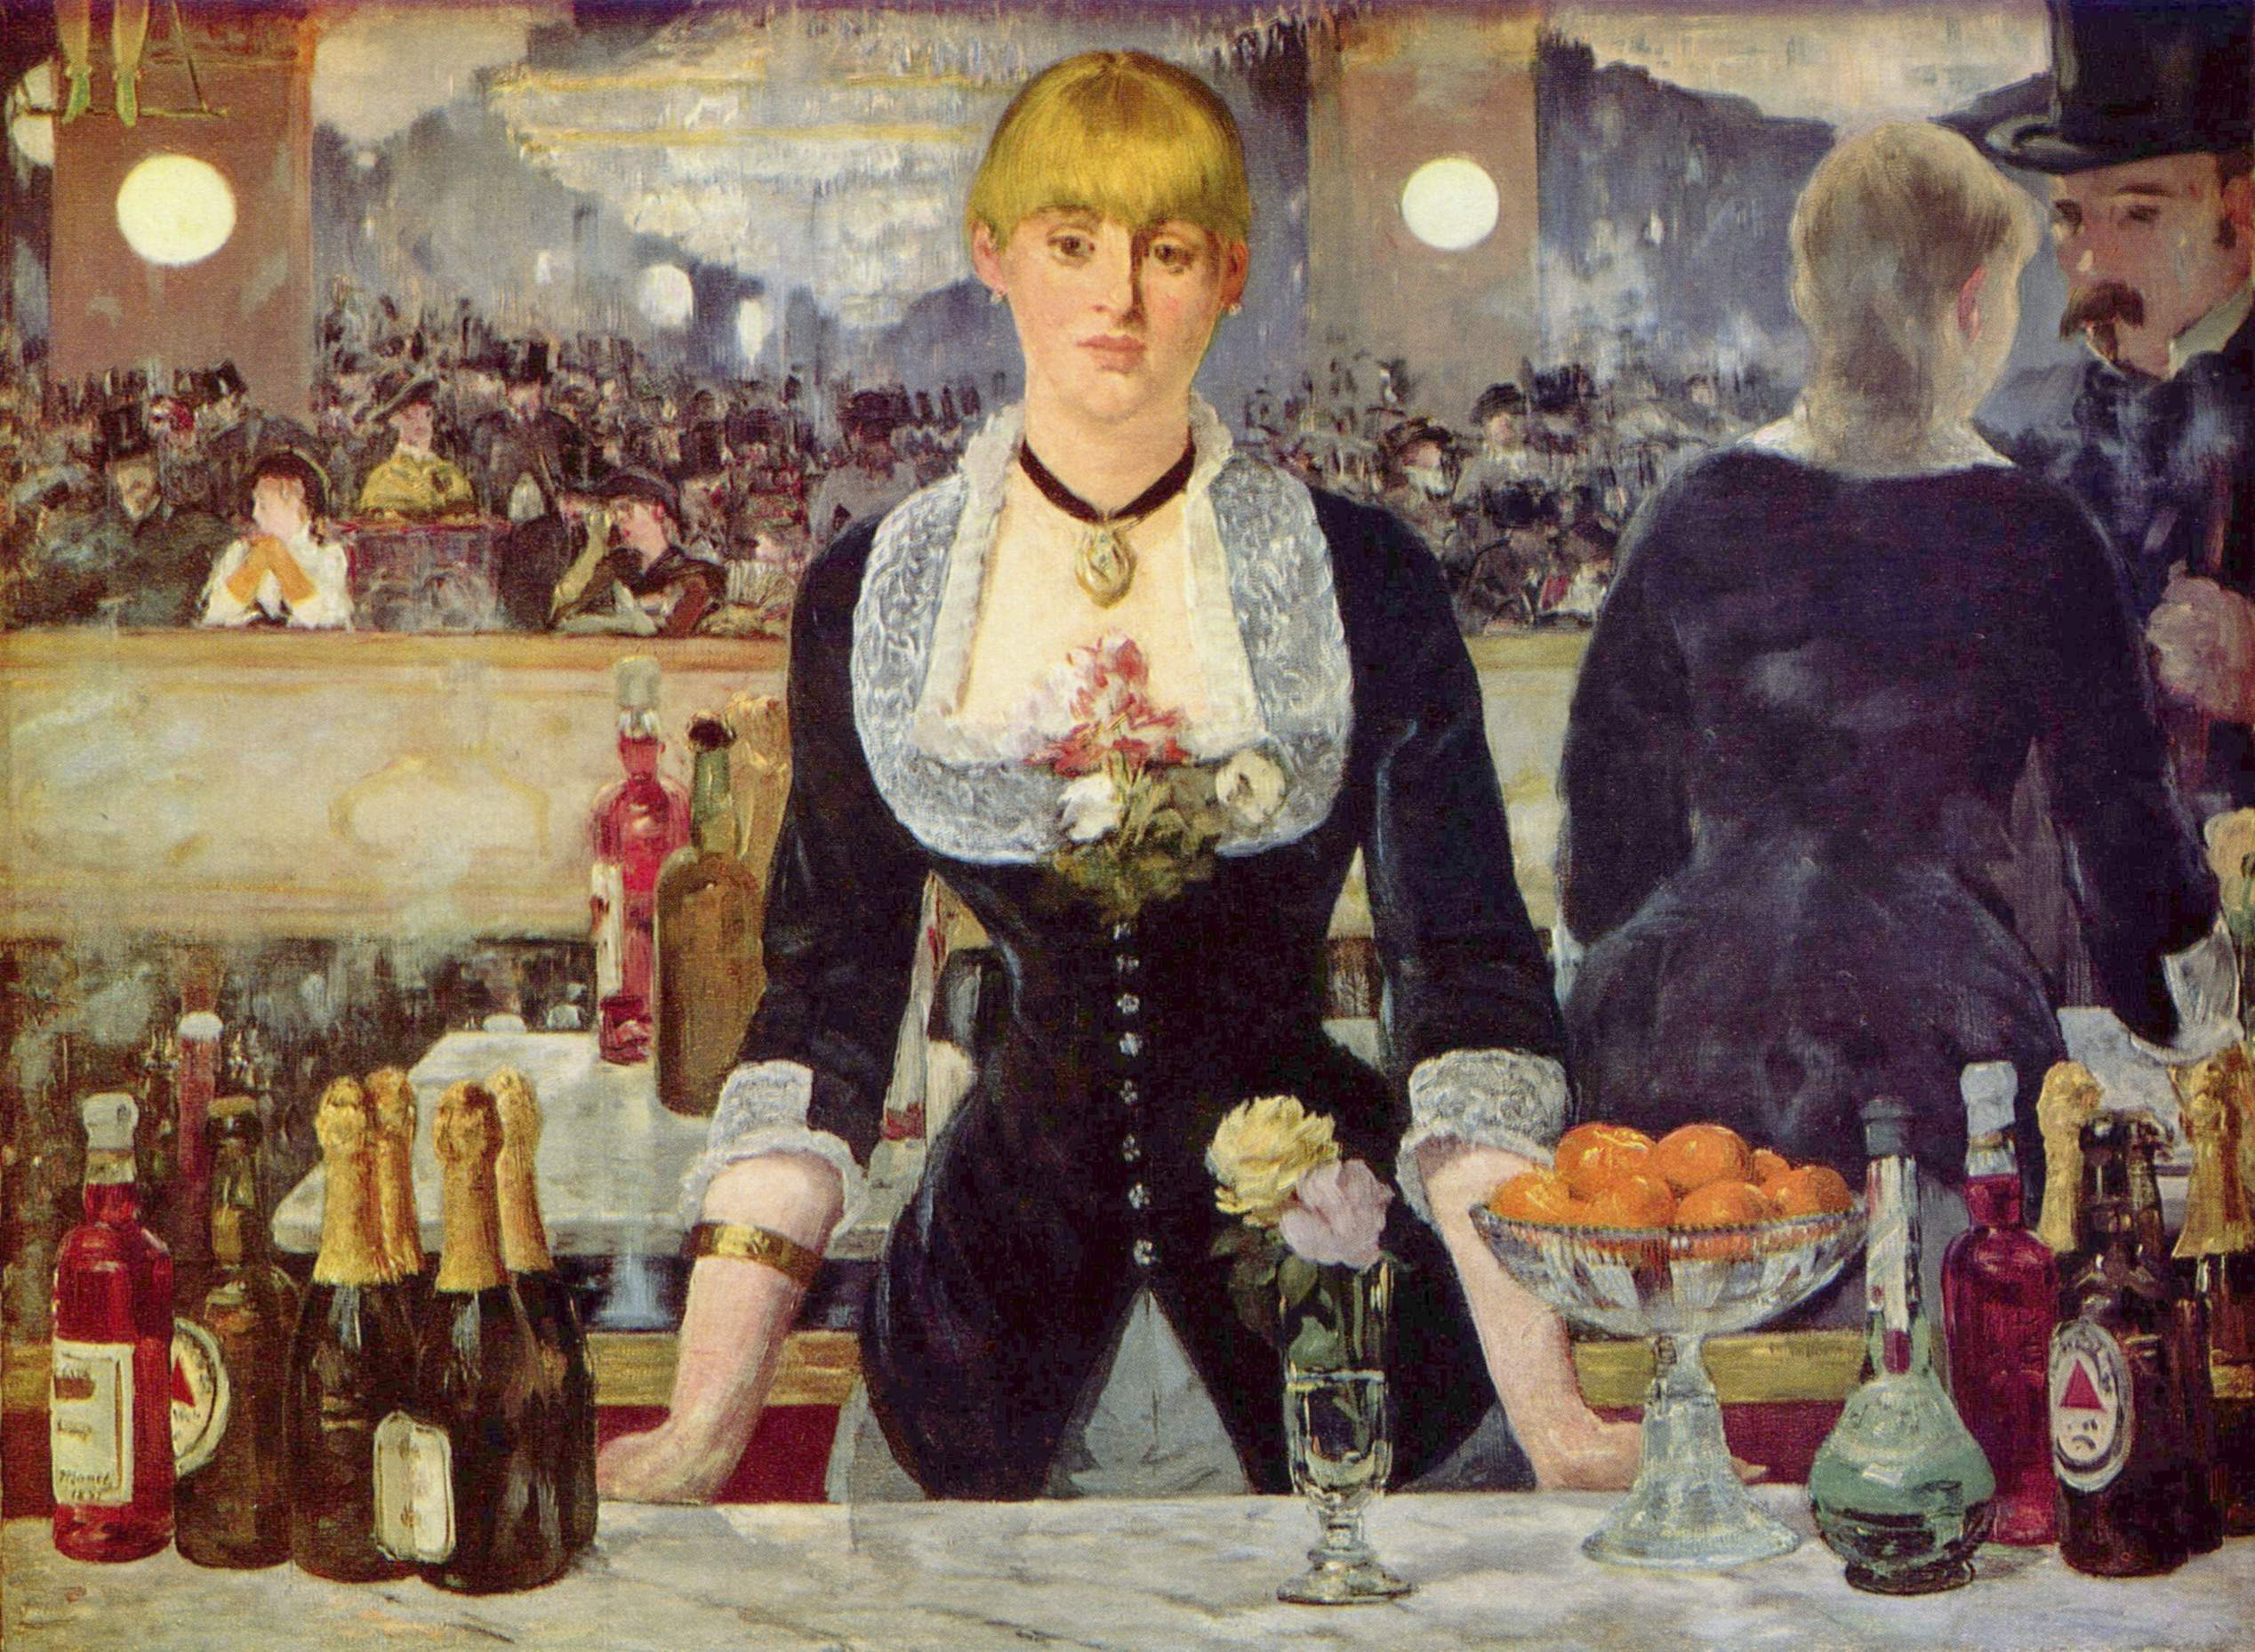
\includegraphics[width=1.25\textwidth]{./chapters/manet}\par
    \par\hfill\hfill{\tiny\bfseries Manet's  \textit{The Barmaid.}}\\
    \par
    \vspace*{\baselineskip}
    \par\hfill},
 title after={\hfill\hfill},
 title font-family=\sffamily,
 title font-color=\color{black!80},
 title font-weight=\bfseries,
 title font-size=\LARGE}}

\cxset{manet}
\chapter{EDOUARD MANET}
\begin{multicols}{3}
      \leftskip0pt
      \lettrine{I}{psum dolor} sit amet latixeus. \lipsum*[1-2]
      Latinicus porcupinus to fill the line.
\end{multicols}

%% CARDINAL

\cxset{manet}

\def\topimage#1{\cxset{title before={\hskip-2.3cm\includegraphics[width=1.25\textwidth]{./chapters/#1}\par
\vspace*{\baselineskip}\par}}}

\cxset{manet}
\topimage{Alan-MacDonald-Cardinal-Spin-01}

\chapter{ALAN MacDONALD}
\begin{multicols}{3}
      \leftskip0pt
      \lettrine{I}{psum dolor} sit amet latixeus. \lipsum*[1-2]
      Latinicus porcupinus to fill the line.
\end{multicols}
\clearpage

This particular code, uses the predefined style \textit{manet}. The only difference we have now defined a helper macro to make it easier for such images to be inserted for similar style chapter openings.

\medskip

\begin{lstlisting}
\def\topimage#1{\cxset{title before={\hskip-2.3cm\includegraphics[width=1.25\textwidth]{./chapters/#1}\par
\vspace*{\baselineskip}\par}}}
\end{lstlisting}

If a full book is to be designed using chapter openings in this fashion more keys and styles could be defined to make it even more easy to enter.

The full code to have the chapter typeset is shown below:
\medskip

\begin{lstlisting}
\cxset{manet}
\topimage{Alan-MacDonald-Cardinal-Spin-01}

\chapter{ALAN MacDONALD}
\begin{multicols}{3}
      \leftskip0pt
      \lettrine{I}{psum dolor} sit amet latixeus. \lipsum*[1-2]
      Latinicus porcupinus to fill the line.
\end{multicols}
\end{lstlisting}



%%%%%%%%%%%%%%%%%%%%%%%%%%%%%%%%%%%%%%%%%%%
%%%%%%  STYLE 01
%%%%%%%%%%%%%%%%%%%%%%%%%%%%%%%%%%%%%%%%%%%
\clearpage

\cxset{
 name={},
 numbering=arabic,
 number font-size=\LARGE,
 number font-family=\rmfamily,
 number font-weight=\bfseries,
 number before=,
 number dot=,
 number after=,
 number position=leftname,
 chapter font-family=\sffamily,
 chapter font-weight=\normalfont,
 chapter font-size=\Large,
 chapter before={\vspace*{20pt}\par},
 chapter after={\hfill\hfill\par},
 chapter color={black!90},
 number color=\color{purple},
 title beforeskip={\vspace*{30pt}},
 title afterskip={\vspace*{40pt}\par},
 title before={},
 title after={},
 title font-family=\sffamily,
 title font-color=\color{purple},
 title font-weight=\bfseries,
 title font-size=\LARGE}

\chapter{Introduction to Style One}



\begin{summary}
This design is simple and its distinguishing characteristic is a short summary at the beginning of the chapter. This is almost like an abstract typeset in italic font without setting the margins in. We provide a \lstinline{summary} environment for convenience. Note the very simple line in the running head to the left of the page number.
\end{summary}

\medskip
\begin{figure}[ht]
\centering
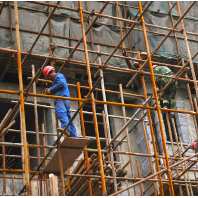
\includegraphics[width=0.5\textwidth]{./chapters/cap3}
\end{figure}



%%%%%%%%%%%%%%%%%%%%%%%%%%%%%%%%%%%%%%%%%%%
%%%%%%  STYLE 02
%%%%%%%%%%%%%%%%%%%%%%%%%%%%%%%%%%%%%%%%%%%
\clearpage

\cxset{
 name={},
 numbering=arabic,
 number font-size=\LARGE,
 number font-family=\rmfamily,
 number font-weight=\bfseries,
 number before=,
 number dot=.,
 number after=\hspace{1em},
 number position=rightname,
 chapter font-family=\sffamily,
 chapter font-weight=\normalfont,
 chapter font-size=\Large,
 chapter before={\vspace*{20pt}\par\hfill},
 chapter after={},
 chapter color={black!90},
 number color=\color{purple},
 title beforeskip={},
 title afterskip={\vspace*{50pt}\par},
 title before={},
 title after={},
 title font-family=\sffamily,
 title font-color=\color{purple},
 title font-weight=\bfseries,
 title font-size=\LARGE}

\chapter{Style 2}
\parindent0pt
I tend to favour this design for books that have a lot of pictures. It brings the design into the margins and leaves plentiful white space in the margins. From a programming point of view the chapter is the opposite of openany. It has to open on an odd number.
\medskip
\begin{figure}[ht]
\centering
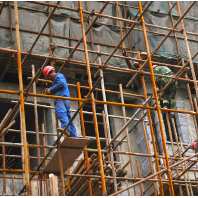
\includegraphics[width=0.6\textwidth]{./chapters/cap3}
\end{figure}

%%%%%%%%%%%%%%%%%%%%%%%%%%%%%%%%%%%%%%%%%%%
%%%%%%  STYLE 03
%%%%%%%%%%%%%%%%%%%%%%%%%%%%%%%%%%%%%%%%%%%
\newgeometry{top=-10pt}
\tcbset{width=\paperwidth,boxrule=0pt,right=3cm,arc=0pt}

\cxset{style03/.style={
 name={},
 numbering=arabic,
 number font-size=\HUGE,
 number font-family=\rmfamily,
 number font-weight=\bfseries,
 number before=,
 number dot=.,
 number after=,
 number position=rightname,
 chapter font-family=\sffamily,
 chapter font-weight=\normalfont,
 chapter font-size=\Large,
% start colorbox
 chapter before={\hspace*{-2.5cm}\vbox\bgroup\tcolorbox\bgroup\vspace*{20pt}\hfill\hfill},
 chapter after={\par\vspace*{15pt}},
 chapter color={black!90},
 number color=\color{purple},
 title beforeskip={},
 title afterskip={\vspace*{10pt}\par},
 title before={\hfill\hfill},
% end colorbox
 title after={\vspace*{60pt}\egroup\endtcolorbox\egroup},
 title font-family=\sffamily,
 title font-color=\color{purple},
 title font-weight=\bfseries,
 title font-size=\Huge}}

\cxset{style03}

\chapter{Introduction Style Three}

This is not an exact reproduction as I am still thinking as to how to use
specials with the package. You can vary it by setting the tcolorbox settings as well as the geometry settings.
\medskip
\begin{figure}[ht]
\centering
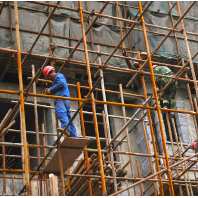
\includegraphics[width=0.39\textwidth]{./chapters/cap3}
\end{figure}

This setting involves changing the geometry of the page as well as adding the chapter name and title in a color box. For this I have used the \lstinline{tcolorbox}. Of course you can use any other shaded environment you feel comfortable with such as mdframed. It is important to set the colorbox parameters.

\begin{lstlisting}
\newgeometry{top=-10pt}
\tcbset{width=\paperwidth,boxrule=0pt,right=3cm,arc=0pt}
\end{lstlisting}

Note that we set the width of the \lstinline{tcolorbox} to \lstinline{\paperwidth} in order for the shading to extend to the full width of the page.

\restoregeometry

%%%%%%%%%%%%%%%%%%%%%%%%%%%%%%%%%%%%%%%%%%%
%%%%%%  STYLE 04
%%%%%%%%%%%%%%%%%%%%%%%%%%%%%%%%%%%%%%%%%%%
\clearpage
\cxset{style04/.style={
 name={},
 numbering=Roman,
 number font-size=\Large,
 number font-family=\rmfamily,
 number font-weight=\bfseries,
 number before=,
 number dot=,
 number after=,
 number position=rightname,
 chapter font-family=\rmfamily,
 chapter font-weight=\normalfont,
 chapter font-size=\Large,
 chapter before={\vspace*{20pt}\par\hfill},
 chapter after={\hfill\hfill\par\vspace*{10pt}},
 chapter color={black!90},
 number color=\color{purple},
 title beforeskip={},
 title afterskip={\vspace*{50pt}\par},
 title before={\hfill},
 title after={\hfill\hfill\par},
 title font-family=\rmfamily,
 title font-color=\color{purple},
 title font-weight=\normalfont,
 title font-size=\LARGE}}

\cxset{style04}

\chapter{INTRODUCTION TO STYLE FOUR}

This is a very simple design applicable perhaps to translations and commentary on older texts.
\medskip
\begin{figure}[ht]
\centering
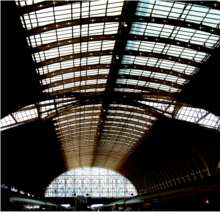
\includegraphics[width=0.6\textwidth]{./chapters/cap3a}
\end{figure}


%%%%%%%%%%%%%%%%%%%%%%%%%%%%%%%%%%%%%%%%%%%
%%%%%%  STYLE 05
%%%%%%%%%%%%%%%%%%%%%%%%%%%%%%%%%%%%%%%%%%%


\cxset{style05/.style={
 name={Chapter},
 numbering=arabic,
 number font-size=\Large,
 number font-family=\rmfamily,
 number font-weight=\normalfont\itshape,
 number color=\color{black!90},
 number before=,
 number dot=,
 number after=,
 number position=rightname,
 chapter font-family=\rmfamily,
 chapter font-weight=\normalfont\itshape,
 chapter font-size=\Large,
 chapter before={\mediumrule\vspace*{20pt}\par\hfill},
 chapter after={\hfill\hfill\par},
 chapter color={black!90},
 chapter spaceout=none,
 title beforeskip={\vspace*{10pt}},
 title afterskip={\vspace*{50pt}\par},
 title before={\hfill},
 title after={\hfill\hfill\par\thinrule},
 title font-family=\sffamily,
 title font-color=\color{black!90},
 title font-weight=\bfseries,
 title font-size=\huge}}

\cxset{style05}
\chapter{Introduction to Style Five}

I think this style can be improved with a bit of color. You can experiment with it quite easily. The spacing on top of this style can also be adjusted to suit your typographical taste.
\medskip
\begin{figure}[ht]
\centering
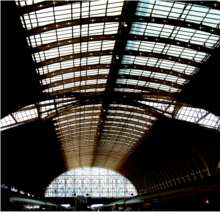
\includegraphics[width=0.6\textwidth]{./chapters/cap3a}
\end{figure}

%%%%%%%%%%%%%%%%%%%%%%%%%%%%%%%%%%%%%%%%%%%
%%%%%%  STYLE 06
%%%%%%%%%%%%%%%%%%%%%%%%%%%%%%%%%%%%%%%%%%%

\cxset{style6/.style={
 name={Chapter},
 numbering=arabic,
 number font-size=\Huge,
 number font-family=\rmfamily,
 number font-weight=\calligra,
 number color=\color{black!90},
 number before=\kern-4.5pt,
 number dot=,
 number after=,
 number position=rightname,
 chapter font-family=\rmfamily,
 chapter font-weight=\normalfont\itshape,
 chapter font-size=\LARGE\calligra,
 chapter before={\vspace*{20pt}\par\hfill},
 chapter after={\hfill\hfill\par},
 chapter color={black!90},
 title beforeskip={\vspace*{50pt}},
 title afterskip={\vspace{20pt}\par},
 title before={\hfill},
 title after={\hfill\hfill},
 title font-family=\rmfamily,
 title font-color=\color{black!90},
 title font-weight=\normalfont,
 title font-size=\LARGE,
 title spaceout=soul,
}}

\cxset{style6}

\chapter{INTRODUCTION TO STYLE SIX}

The calligraphic font for this design make it stand out, although you may need to experiment to get the right font (I have used calligra). I am sure the specification can be optimized a bit, however so far it works. I also opted to space out the title.
\medskip
\begin{figure}[ht]
\centering
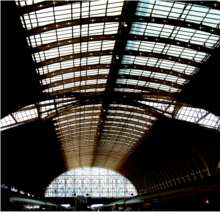
\includegraphics[width=0.6\textwidth]{./chapters/cap3a}
\end{figure}

The number has been kerned using:

\begin{lstlisting}
 number before=\kern-4.5pt,
\end{lstlisting}


%%%%%%%%%%%%%%%%%%%%%%%%%%%%%%%%%%%%%%%%%%%
%%%%%%  STYLE 07
%%%%%%%%%%%%%%%%%%%%%%%%%%%%%%%%%%%%%%%%%%%

\cxset{style7/.style={
 name={},
 numbering=arabic,
 number font-size=\Huge,
 number font-family=\rmfamily,
 number font-weight=\bfseries,
 number before=,
 number dot=,
 number color=\color{gray},
 number after=\par,
 number position=rightname,
 chapter font-family=\sffamily,
 chapter font-weight=\normalfont,
 chapter font-size=\Large,
 chapter before={\hfill\hfill\par},
 chapter after={},
 chapter color={black!90},
 title beforeskip={\vspace*{30pt}},
 title afterskip={\vspace*{50pt}\par},
 title before={},
 title after={\par\rule[13pt]{\textwidth}{0.4pt}},
 title font-family=\sffamily,
 title font-color=\color{purple},
 title font-weight=\bfseries,
 title font-size=\LARGE,
 title spaceout=none,
}}

\cxset{style7}
\chapter{Introduction to Style Seven}

\parindent0pt
\lipsum[1]
\medskip
\begin{figure}[ht]
\centering
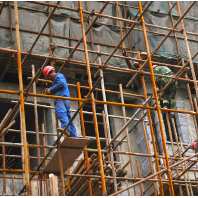
\includegraphics[width=0.6\textwidth]{./chapters/cap3}
\end{figure}
\lipsum[1]


%%%%%%%%%%%%%%%%%%%%%%%%%%%%%%%%%%%%%%%%%%%
%%%%%%  STYLE 08
%%%%%%%%%%%%%%%%%%%%%%%%%%%%%%%%%%%%%%%%%%%
\clearpage

\cxset{style8/.style={
 name={},
 numbering=arabic,
 number font-size=\LARGE,
 number font-family=\sffamily,
 number font-weight=\bfseries,
 number color=\color{black!90},
 number before=,
 number dot=,
 number after=,
 number position=rightname,
 chapter font-family=\sffamily,
 chapter font-weight=\normalfont,
 chapter font-size=\Large,
 chapter before={\vspace*{20pt}\hfill},
 chapter after={\vspace{20pt}\par},
 chapter color={black!90},
 title beforeskip={},
 title afterskip={\vspace*{50pt}\par},
 title before={\hfill\hfill\raggedleft},
 title after={},
 title font-family=\sffamily,
 title font-color=\color{black!90},
 title font-weight=\bfseries,
 title font-size=\LARGE}}

\cxset{style8}
\chapter[Introduction to Style Eight]{Introduction to Chapter\\ Style Eight\\[20pt]
{\small\normalfont Dr Yiannis Lazarides\\[-10pt] Larnaka, Cyprus}}

\lipsum[1]
\medskip
\begin{figure}[ht]
\centering
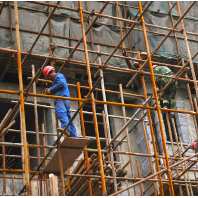
\includegraphics[width=0.5\textwidth]{./chapters/cap3}
\end{figure}
\lipsum[1]



%%%%%%%%%%%%%%%%%%%%%%%%%%%%%%%%%%%%%%%%%%%
%%%%%%  STYLE 09
%%%%%%%%%%%%%%%%%%%%%%%%%%%%%%%%%%%%%%%%%%%
\clearpage

\cxset{
 name={},
 numbering=arabic,
 number font-size=\LARGE,
 number font-family=\rmfamily,
 number font-weight=\bfseries,
 number before=,
 number dot=.,
 number after=\hspace{1em},
 number position=rightname,
 chapter font-family=\sffamily,
 chapter font-weight=\normalfont,
 chapter font-size=\Large,
 chapter before={\vspace*{20pt}\par\hfill},
 chapter after={},
 chapter color={black!90},
 number color=\color{purple},
 title beforeskip={},
 title afterskip={\vspace*{50pt}\par},
 title before={},
 title after={},
 title font-family=\sffamily,
 title font-color=\color{purple},
 title font-weight=\bfseries,
 title font-size=\LARGE}
\chapter{Introduction 09}
\lipsum[1]

\medskip
\begin{figure}[ht]
\centering
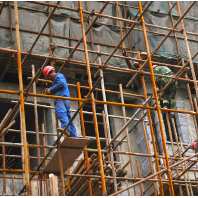
\includegraphics[width=0.8\textwidth]{./chapters/cap3}
\end{figure}

\textit{In preparation. Patience!}

%%%%%%%%%%%%%%%%%%%%%%%%%%%%%%%%%%%%%%%%%%%
%%%%%%  STYLE 10
%%%%%%%%%%%%%%%%%%%%%%%%%%%%%%%%%%%%%%%%%%%

\cxset{
 name={},
 numbering=arabic,
 number font-size=\LARGE,
 number font-family=\rmfamily,
 number font-weight=\bfseries,
 number before=,
 number dot=.,
 number after=\hspace{1em},
 number position=rightname,
 chapter font-family=\sffamily,
 chapter font-weight=\normalfont,
 chapter font-size=\Large,
 chapter before={\vspace*{20pt}\par\hfill},
 chapter after={},
 chapter color={black!90},
 number color=\color{purple},
 title beforeskip={},
 title afterskip={\vspace*{50pt}\par},
 title before={},
 title after={},
 title font-family=\sffamily,
 title font-color=\color{purple},
 title font-weight=\bfseries,
 title font-size=\LARGE}
\chapter{Introduction 10}
\lipsum[1]

\medskip
\begin{figure}[ht]
\centering
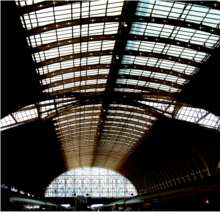
\includegraphics[width=0.6\textwidth]{./chapters/cap3a}
\end{figure}

\lipsum[1]


%%%%%%%%%%%%%%%%%%%%%%%%%%%%%%%%%%%%%%%%%%%
%%%%%%  STYLE 11
%%%%%%%%%%%%%%%%%%%%%%%%%%%%%%%%%%%%%%%%%%%

\cxset{style11/.style={
 name={Chapter},
 numbering=arabic,
 number font-size=\LARGE,
 number font-family=\rmfamily,
 number font-weight=\bfseries,
 number before=,
 number dot=,
 number after=,
 number position=rightname,
 chapter font-family=\rmfamily,
 chapter font-weight=\bfseries,
 chapter font-size=\LARGE,
 chapter before={\vspace*{20pt}\par\hfill},
 chapter after={\hfill\hfill\par\vspace{10pt}},
 chapter color={black!90},
 number color=\color{black!90},
 title beforeskip={},
 title afterskip={\vspace*{20pt}\par},
 title before={\hfill},
 title after={\hfill\hfill\par},
 title font-family=\rmfamily,
 title font-color=\color{black!90},
 title font-weight=\bfseries,
 title font-size=\LARGE}}

\cxset{style11}
\chapter{Introduction to Style Eleven}
\lipsum[2]

\medskip
\begin{figure}[ht]
\centering
\fbox{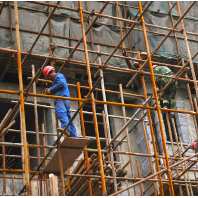
\includegraphics[width=0.65\textwidth]{./chapters/cap3}}
\end{figure}
\lipsum[1]

%%%%%%%%%%%%%%%%%%%%%%%%%%%%%%%%%%%%%%%%%%%
%%%%%%  STYLE 12
%%%%%%%%%%%%%%%%%%%%%%%%%%%%%%%%%%%%%%%%%%%
\cxset{style12/.style={
 name={},
 numbering=arabic,
 number font-size=\HUGE,
 number font-family=\rmfamily,
 number font-weight=\bfseries,
 number before=,
 number dot=,
 number color=\color{gray},
 number after=\par,
 number position=rightname,
 chapter font-family=\sffamily,
 chapter font-weight=\normalfont,
 chapter font-size=\Huge,
 chapter before={\raggedright\par},
 chapter after={},
 chapter color={black!90},
 title beforeskip={\vspace*{30pt}},
 title afterskip={\vspace*{50pt}\par},
 title before={},
 title after={\par\vspace{30pt}\rule{\textwidth}{4pt}},
 title font-family=\sffamily,
 title font-color=\color{purple},
 title font-weight=\bfseries,
 title font-size=\HUGE,
 title spaceout=none,
}}


\cxset{style12}
\chapter{Introduction to \\ Style Twelve}

This is a variation of Style 7, with only the lettering and the rule are thicker. In my opinion it looks better with a bit of color, so I have used a purple color with a gray.

\medskip
\begin{figure}[ht]
\centering
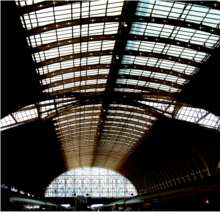
\includegraphics[width=0.35\textwidth]{./chapters/cap3a}
\end{figure}
\lipsum[1]

%%%%%%%%%%%%%%%%%%%%%%%%%%%%%%%%%%%%%%%%%%%
%%%%%%  STYLE 13
%%%%%%%%%%%%%%%%%%%%%%%%%%%%%%%%%%%%%%%%%%%

\cxset{style13/.style={
 name={Chapter},
 numbering=arabic,
 number font-size=\HUGE,
 number font-family=\sffamily,
 number font-weight=\bfseries,
 number color=\color{gray!50},
 number before=\par\vspace*{5pt}\hfill\hfill,
 number dot=,
 number after={\hspace*{7pt}\par},
 number position=rightname,
 chapter font-family=\sffamily,
 chapter font-weight=\normalfont,
 chapter font-size=\LARGE,
 chapter before={\thinrule\vspace*{20pt}\par\hfill\hfill},
 chapter after={\vskip0pt\par},
 chapter color={black!50},
 title beforeskip={\vspace*{10pt}},
 title afterskip={\vspace*{50pt}\par},
 title before={\hfill\hfill\raggedleft},
 title after={},
 title font-family=\sffamily,
 title font-color=\color{purple},
 title font-weight=\bfseries,
 title font-size=\huge}}

\cxset{style13}

\chapter{Introduction to Chapter\\ Style Thirteen}
\lipsum[1]
\medskip
\begin{figure}[ht]
\centering
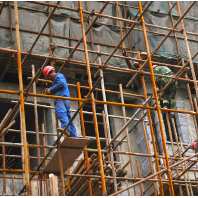
\includegraphics[width=0.45\textwidth]{./chapters/cap3}
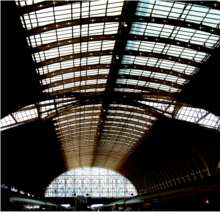
\includegraphics[width=0.45\textwidth]{./chapters/cap3a}
\end{figure}
\lipsum[2]


%%%%%%%%%%%%%%%%%%%%%%%%%%%%%%%%%%%%%%%%%%%
%%%%%%  STYLE 14
%%%%%%%%%%%%%%%%%%%%%%%%%%%%%%%%%%%%%%%%%%%
\clearpage

\cxset{
 name={},
 numbering=arabic,
 number font-size=\LARGE,
 number font-family=\rmfamily,
 number font-weight=\bfseries,
 number before=,
 number dot=.,
 number after=\hspace{1em},
 number position=rightname,
 chapter font-family=\sffamily,
 chapter font-weight=\normalfont,
 chapter font-size=\Large,
 chapter before={\vspace*{20pt}\par\hfill},
 chapter after={},
 chapter color={black!90},
 number color=\color{purple},
 title beforeskip={},
 title afterskip={\vspace*{50pt}\par},
 title before={},
 title after={},
 title font-family=\sffamily,
 title font-color=\color{purple},
 title font-weight=\bfseries,
 title font-size=\LARGE}
\chapter{Introduction 14}
\lipsum[1]
\medskip
\begin{figure}[ht]
\centering
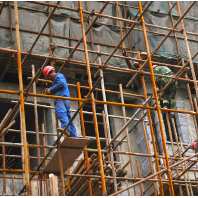
\includegraphics[width=0.65\textwidth]{./chapters/cap3}
\end{figure}
\lipsum[2]

%%%%%%%%%%%%%%%%%%%%%%%%%%%%%%%%%%%%%%%%%%%
%%%%%%  STYLE 15
%%%%%%%%%%%%%%%%%%%%%%%%%%%%%%%%%%%%%%%%%%%

\cxset{
 name={},
 numbering=arabic,
 number font-size=\LARGE,
 number font-family=\rmfamily,
 number font-weight=\bfseries,
 number before=,
 number dot=.,
 number after=\hspace{1em},
 number position=rightname,
 chapter font-family=\sffamily,
 chapter font-weight=\normalfont,
 chapter font-size=\Large,
 chapter before={\vspace*{20pt}\par\hfill},
 chapter after={},
 chapter color={black!90},
 number color=\color{purple},
 title beforeskip={},
 title afterskip={\vspace*{50pt}\par},
 title before={},
 title after={},
 title font-family=\sffamily,
 title font-color=\color{purple},
 title font-weight=\bfseries,
 title font-size=\LARGE}
\chapter{Introduction 15}
\lipsum[1]
\medskip
\begin{figure}[ht]
\centering
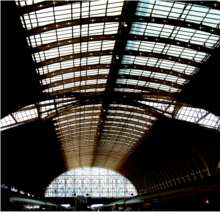
\includegraphics[width=0.65\textwidth]{./chapters/cap3a}
\end{figure}
\lipsum[2]

%%%%%%%%%%%%%%%%%%%%%%%%%%%%%%%%%%%%%%%%%%%
%%%%%%  STYLE 16
%%%%%%%%%%%%%%%%%%%%%%%%%%%%%%%%%%%%%%%%%%%
\cxset{
 name={},
 numbering=arabic,
 number font-size=\LARGE,
 number font-family=\rmfamily,
 number font-weight=\bfseries,
 number before=,
 number dot=.,
 number after=\hspace{1em},
 number position=rightname,
 chapter font-family=\sffamily,
 chapter font-weight=\normalfont,
 chapter font-size=\Large,
 chapter before={\vspace*{20pt}\par\hfill},
 chapter after={},
 chapter color={black!90},
 number color=\color{purple},
 title beforeskip={},
 title afterskip={\vspace*{50pt}\par},
 title before={},
 title after={},
 title font-family=\sffamily,
 title font-color=\color{purple},
 title font-weight=\bfseries,
 title font-size=\LARGE}
\chapter{Introduction 16}
\lipsum[1]
\medskip
\begin{figure}[ht]
\centering
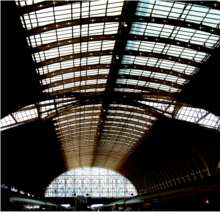
\includegraphics[width=0.65\textwidth]{./chapters/cap3a}
\end{figure}
\lipsum[2]

%%%%%%%%%%%%%%%%%%%%%%%%%%%%%%%%%%%%%%%%%%%
%%%%%%  STYLE 17
%%%%%%%%%%%%%%%%%%%%%%%%%%%%%%%%%%%%%%%%%%%

\cxset{style17/.style={
 name={},
 numbering=arabic,
 number font-size=\LARGE,
 number font-family=\sffamily,
 number font-weight=\bfseries,
 number before=,
 number dot=.,
 number after=\thinspace,
 number position=rightname,
 chapter font-family=\sffamily,
 chapter font-weight=\bfseries,
 chapter font-size=\LARGE,
 chapter before={\vspace*{20pt}\par\hfill},
 chapter after={},
 chapter color={black!90},
 title beforeskip={},
 title afterskip={\vspace*{70pt}\par},
 title before={},
 title after={},
 title font-family=\sffamily,
 title font-color=\color{purple},
 title font-weight=\bfseries,
 title font-size=\LARGE}}
\cxset{style17}
\chapter{Introduction to Style Seventeen}

\lipsum[1]
\medskip
\begin{figure}[ht]
\centering
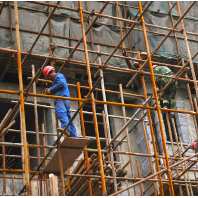
\includegraphics[width=0.5\textwidth]{./chapters/cap3}
\end{figure}
\lipsum[2-4]

%%%%%%%%%%%%%%%%%%%%%%%%%%%%%%%%%%%%%%%%%%%
%%%%%%  STYLE 18
%%%%%%%%%%%%%%%%%%%%%%%%%%%%%%%%%%%%%%%%%%%

\cxset{
 name={},
 numbering=arabic,
 number font-size=\LARGE,
 number font-family=\rmfamily,
 number font-weight=\bfseries,
 number before=\par\hangindent2em\hangafter1,
 number after=\hspace{1em},
 number position=rightname,
 chapter font-family=\sffamily,
 chapter font-weight=\normalfont,
 chapter font-size=\Large,
 chapter before={\vspace*{20pt}},
 chapter after={},
 chapter color={black!90},
 number color=\color{black!90},
 title beforeskip={},
 title afterskip={\vspace*{50pt}\par},
 title before={},
 title after={},
 title font-family=\sffamily,
 title font-color=\color{black},
 title font-weight=\bfseries,
 title font-size=\LARGE}
\chapter{Introduction to chapter\\ style eighteen}

\parindent0pt
I tend to favour this design for books that have a lot of pictures. It brings the design into the margins and leaves plentiful white space in the margins. From a programming point of view the chapter is the opposite of openany. It has to open on an odd number.
\medskip
\begin{figure}[ht]
\centering
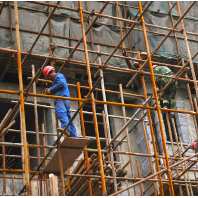
\includegraphics[width=0.65\textwidth]{./chapters/cap3}
\end{figure}

%%%%%%%%%%%%%%%%%%%%%%%%%%%%%%%%%%%%%%%%%%%
%%%%%%  STYLE 19
%%%%%%%%%%%%%%%%%%%%%%%%%%%%%%%%%%%%%%%%%%%


\cxset{
 name={},
 numbering=arabic,
 number font-size=\LARGE,
 number font-family=\rmfamily,
 number font-weight=\bfseries,
 number before=\par\hangindent2em\hangafter1,
 number after=\hspace{1em},
 number position=rightname,
 chapter font-family=\sffamily,
 chapter font-weight=\normalfont,
 chapter font-size=\Large,
 chapter before={\vspace*{20pt}},
 chapter after={},
 chapter color={black!90},
 number color=\color{black!90},
 title beforeskip={},
 title afterskip={\vspace*{50pt}\par},
 title before={},
 title after={},
 title font-family=\sffamily,
 title font-color=\color{black},
 title font-weight=\bfseries,
 title font-size=\LARGE}
\chapter{Introduction to chapter\\ style nineteen}
\lipsum[1]

\medskip
\begin{figure}[ht]
\centering
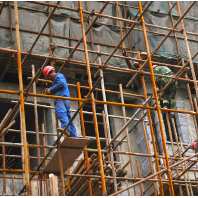
\includegraphics[width=0.65\textwidth]{./chapters/cap3}
\end{figure}

\lipsum[1]

%%%%%%%%%%%%%%%%%%%%%%%%%%%%%%%%%%%%%%%%%%%
%%%%%%  STYLE 21
%%%%%%%%%%%%%%%%%%%%%%%%%%%%%%%%%%%%%%%%%%%

\cxset{
 name={},
 numbering=none,
 number font-size=\Large,
 number font-family=\rmfamily,
 number font-weight=\bfseries,
 number before={},
 number after={},
 number position=rightname,
 chapter font-family=\sffamily,
 chapter font-weight=\normalfont,
 chapter font-size=\Large,
 chapter before={\vspace*{0.3\textheight}},
 chapter after={\par},
 chapter color={black!90},
 number color=\color{black!90},
 title beforeskip={},
 title afterskip={\par\rule{\textwidth}{3.5pt}\vspace{20pt}},
 title before={},
 title after={},
 title font-family=\sffamily,
 title font-color=\color{black},
 title font-weight=\bfseries,
 title font-size=\Huge}
\chapter{INTRODUCTION TO STYLE 21}

\lipsum[1]
\medskip
\begin{figure}[ht]
\centering
\fbox{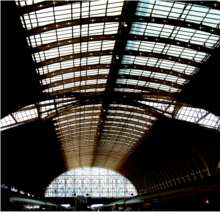
\includegraphics[width=0.65\textwidth]{./chapters/cap3a}}
\end{figure}
\lipsum[1]

%%%%%%%%%%%%%%%%%%%%%%%%%%%%%%%%%%%%%%%%%%%
%%%%%%  STYLE 22
%%%%%%%%%%%%%%%%%%%%%%%%%%%%%%%%%%%%%%%%%%%

\newgeometry{left=2.5in}
\cxset{
 name={},
 numbering=none,
 number font-size=\Large,
 number font-family=\rmfamily,
 number font-weight=\bfseries,
 number before={},
 number after={},
 number position=rightname,
 chapter font-family=\sffamily,
 chapter font-weight=\normalfont,
 chapter font-size=\Large,
 chapter before={\vspace*{-80pt}},
 chapter after={\par},
 chapter color={black!90},
 number color=\color{black!90},
 title beforeskip={\hfill},
 title afterskip={\vspace{70pt}},
 title before=\hspace*{-1in},
 title after={},
 title font-family=\sffamily,
 title font-color=\color{black},
 title font-weight=\bfseries,
 title font-size=\huge}

\chapter{INTRODUCTION TO STYLE TWENTY TWO}

\section*{INTRODUCTION}

\lettrine{Y}{annis}. \lipsum[2]

\medskip
\begin{figure}[ht]
\centering
\fbox{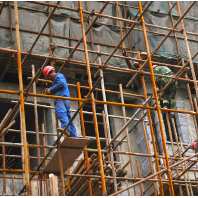
\includegraphics[width=0.5\textwidth]{./chapters/cap3}}
\end{figure}

\lipsum[1-2]


%%%%%%%%%%%%%%%%%%%%%%%%%%%%%%%%%%%%%%%%%%%
%%%%%%  STYLE 23
%%%%%%%%%%%%%%%%%%%%%%%%%%%%%%%%%%%%%%%%%%%
\restoregeometry

\cxset{
 name={Chapter},
 numbering=arabic,
 number font-size=\Large,
 number font-family=\rmfamily,
 number font-weight=\bfseries,
 number before={},
 number after={},
 number position=rightname,
 chapter font-family=\sffamily,
 chapter font-weight=\normalfont,
 chapter font-size=\Large,
 chapter before={\rule{\textwidth}{0.4pt}\par},
 chapter after={\par},
 chapter color={black!90},
 number color=\color{black!90},
 title beforeskip={},
 title afterskip={\vspace{30pt}},
 title before=,
 title after={\par\rule{\textwidth}{0.4pt}\par},
 title font-family=\rmfamily,
 title font-color=\color{black!80},
 title font-weight=\bfseries,
 title font-size=\LARGE}
\chapter{Introduction to style twenty three}

The interesting part of this style is that it uses roman numerals to display the counter that is in a different font than that used for the chapter name.
\medskip
\begin{figure}[ht]
\centering
\fbox{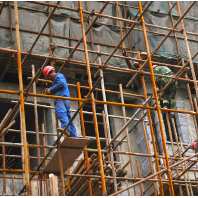
\includegraphics[width=0.5\textwidth]{./chapters/cap3}}
\end{figure}
\lipsum[2-3]



%%%%%%%%%%%%%%%%%%%%%%%%%%%%%%%%%%%%%%%%%%%
%%%%%%  STYLE 24
%%%%%%%%%%%%%%%%%%%%%%%%%%%%%%%%%%%%%%%%%%%
\clearpage
\cxset{
 name={},
 numbering=arabic,
 number font-size=\huge,
 number font-family=\sffamily,
 number font-weight=\bfseries,
 number before={},
 number position=leftname,
 chapter font-family=\sffamily,
 chapter font-weight=\normalfont,
 chapter font-size=\small,
 number after={},
 chapter before={},
 chapter after={\par\vskip12pt},
 chapter color={black!90},
 number color=\color{black!90},
 title beforeskip={},
 title afterskip={\vspace{30pt}},
 title before=,
 title after={\par},
 title font-family=\sffamily,
 title font-color=\color{black!80},
 title font-weight=\bfseries,
 title font-size=\LARGE}
\chapter{Introduction to style twenty four\\{\bfseries\small\itshape Dr. Yiannis Lazarides and Athena Lazarides}}

The interesting part of this style is that it uses roman numerals to display the counter that is in a different font than that used for the chapter name.
\medskip
\begin{figure}[ht]
\centering
\fbox{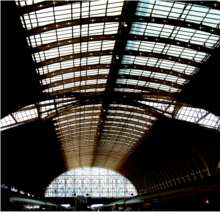
\includegraphics[width=0.6\textwidth]{./chapters/cap3a}}
\end{figure}
\lipsum[2-3]


%%%%%%%%%%%%%%%%%%%%%%%%%%%%%%%%%%%%%%%%%%%
%%%%%%  STYLE 25
%%%%%%%%%%%%%%%%%%%%%%%%%%%%%%%%%%%%%%%%%%%

\cxset{
 name={},
 numbering=arabic,
 number font-size=\huge,
 number font-family=\sffamily,
 number font-weight=\bfseries,
 number before={},
 number position=leftname,
 chapter font-family=\sffamily,
 chapter font-weight=\normalfont,
 chapter font-size=\small,
 number after={},
 chapter before={},
 chapter after={\par\vskip12pt},
 chapter color={black!90},
 number color=\color{black!90},
 title beforeskip={},
 title afterskip={\vspace{30pt}},
 title before=,
 title after={\par},
 title font-family=\sffamily,
 title font-color=\color{black!80},
 title font-weight=\bfseries,
 title font-size=\LARGE}
\chapter{Introduction to style twenty five\\{\bfseries\small\itshape Dr. Yiannis Lazarides and Athena Lazarides}}

The interesting part of this style is that it uses roman numerals to display the counter that is in a different font than that used for the chapter name.
\medskip
\begin{figure}[ht]
\centering
\fbox{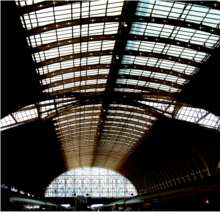
\includegraphics[width=0.5\textwidth]{./chapters/cap3a}}
\end{figure}
\lipsum[1-2]

%%%%%%%%%%%%%%%%%%%%%%%%%%%%%%%%%%%%%%%%%%%
%%%%%%  STYLE 26
%%%%%%%%%%%%%%%%%%%%%%%%%%%%%%%%%%%%%%%%%%%

\cxset{
 name={},
 numbering=arabic,
 number font-size=\huge,
 number font-family=\sffamily,
 number font-weight=\bfseries,
 number before={},
 number position=leftname,
 chapter font-family=\sffamily,
 chapter font-weight=\normalfont,
 chapter font-size=\small,
 number after={},
 chapter before={},
 chapter after={\par\vskip12pt},
 chapter color={black!90},
 number color=\color{black!90},
 title beforeskip={},
 title afterskip={\vspace{30pt}},
 title before=,
 title after={\par},
 title font-family=\sffamily,
 title font-color=\color{black!80},
 title font-weight=\bfseries,
 title font-size=\LARGE}
\chapter{Introduction to style twenty five\\{\bfseries\small\itshape Dr. Yiannis Lazarides and Athena Lazarides}}

The interesting part of this style is that it uses roman numerals to display the counter that is in a different font than that used for the chapter name.
\medskip
\begin{figure}[ht]
\centering
\fbox{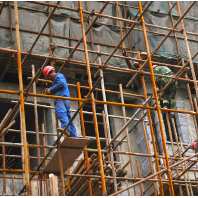
\includegraphics[width=0.6\textwidth]{./chapters/cap3}}
\end{figure}
\lipsum[2-3]


%%%%%%%%%%%%%%%%%%%%%%%%%%%%%%%%%%%%%%%%%%%
%%%%%%  STYLE 27
%%%%%%%%%%%%%%%%%%%%%%%%%%%%%%%%%%%%%%%%%%%

\cxset{
 name={},
 numbering=arabic,
 number font-size=\HUGE,
 number font-family=\sffamily,
 number font-weight=\bfseries,
 number before={},
 number dot=,
 number position=leftname,
 chapter font-family=\sffamily,
 chapter font-weight=\normalfont,
 chapter font-size=\small,
 number after={},
 chapter before={\vspace*{50pt}},
 chapter after={\par\vskip12pt},
 chapter color={black!90},
 number color=\color{black!90},
 title beforeskip={},
 title afterskip={\vspace{30pt}},
 title before=,
 title after={\par},
 title font-family=\sffamily,
 title font-color=\color{black!80},
 title font-weight=\bfseries,
 title font-size=\huge}
\chapter{Introduction to style twenty seven\\{\bfseries\small\itshape Dr. Yiannis Lazarides and Athena Lazarides}}
\lipsum[3]

\medskip
\begin{figure}[ht]
\centering
\fbox{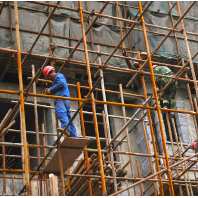
\includegraphics[width=0.5\textwidth]{./chapters/cap3}}
\end{figure}
\lipsum[2-3]


%%%%%%%%%%%%%%%%%%%%%%%%%%%%%%%%%%%%%%%%%%%
%%%%%%  STYLE 28
%%%%%%%%%%%%%%%%%%%%%%%%%%%%%%%%%%%%%%%%%%%

\cxset{
 name={},
 numbering=arabic,
 number font-size=\HUGE,
 number font-family=\sffamily,
 number font-weight=\bfseries,
 number before={},
 number position=leftname,
 chapter font-family=\sffamily,
 chapter font-weight=\normalfont,
 chapter font-size=\small,
 number after={},
 chapter before={},
 chapter after={\hspace*{20pt}},
 chapter color={black!90},
 number color=\color{black!90},
 title beforeskip={},
 title afterskip={\vspace{70pt}},
 title before=,
 title after={\par},
 title font-family=\itshape,
 title font-color=\color{black!80},
 title font-weight=\itshape,
 title font-size=\LARGE}
\chapter{Introduction to Style Twenty Eight}

The interesting part of this style is that it uses roman numerals to display the counter that is in a different font than that used for the chapter name.
\medskip
\begin{figure}[ht]
\centering
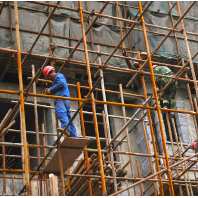
\includegraphics[width=0.6\textwidth]{./chapters/cap3}
\end{figure}
\lipsum[2]

%%%%%%%%%%%%%%%%%%%%%%%%%%%%%%%%%%%%%%%%%%%
%%%%%%  STYLE 29
%%%%%%%%%%%%%%%%%%%%%%%%%%%%%%%%%%%%%%%%%%%
 \cxset{
 name={},
 numbering=arabic,
 number font-size=\HUGE,
 number font-family=\sffamily,
 number font-weight=\bfseries,
 number before={},
 number position=leftname,
 chapter font-family=\sffamily,
 chapter font-weight=\normalfont,
 chapter font-size=\small,
 number after={},
 chapter before={},
 chapter after={\hspace*{20pt}},
 chapter color={black!90},
 number color=\color{black!90},
 title beforeskip={},
 title afterskip={\vspace{70pt}},
 title before=,
 title after={\par},
 title font-family=\itshape,
 title font-color=\color{black!80},
 title font-weight=\itshape,
 title font-size=\LARGE}
\chapter{Introduction to Style Twenty Nine}

The interesting part of this style is that it uses roman numerals to display the counter that is in a different font than that used for the chapter name.
\medskip
\begin{figure}[ht]
\centering
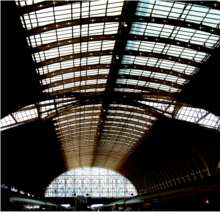
\includegraphics[width=0.6\textwidth]{./chapters/cap3a}
\end{figure}
\lipsum[3]

%%%%%%%%%%%%%%%%%%%%%%%%%%%%%%%%%%%%%%%%%%%
%%%%%%  STYLE 30
%%%%%%%%%%%%%%%%%%%%%%%%%%%%%%%%%%%%%%%%%%%

\cxset{
 name={},
 numbering=arabic,
 number font-size=\HUGE,
 number font-family=\sffamily,
 number font-weight=\bfseries,
 number before={},
 number position=leftname,
 chapter font-family=\sffamily,
 chapter font-weight=\normalfont,
 chapter font-size=\small,
 number after={},
 chapter before={},
 chapter after={\hspace*{20pt}},
 chapter color={black!90},
 number color=\color{black!90},
 title beforeskip={},
 title afterskip={\vspace{70pt}},
 title before=,
 title after={\par},
 title font-family=\itshape,
 title font-color=\color{black!80},
 title font-weight=\itshape,
 title font-size=\LARGE}
\chapter{Introduction to Style Thirty}

The interesting part of this style is that it uses roman numerals to display the counter that is in a different font than that used for the chapter name.
\medskip
\begin{figure}[ht]
\centering
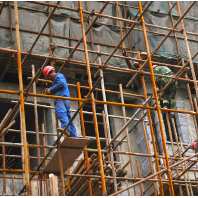
\includegraphics[width=0.6\textwidth]{./chapters/cap3}
\end{figure}



%%%%%%%%%%%%%%%%%%%%%%%%%%%%%%%%%%%%%%%%%%%
%%%%%%  STYLE 31
%%%%%%%%%%%%%%%%%%%%%%%%%%%%%%%%%%%%%%%%%%%

\cxset{
 name={},
 numbering=arabic,
 number font-size=\HUGE,
 number font-family=\sffamily,
 number font-weight=\bfseries,
 number before={\hspace*{-30pt}},
 number position=leftname,
 chapter font-family=\sffamily,
 chapter font-weight=\normalfont,
 chapter font-size=\small,
 number after={},
 chapter before={\hspace*{-30pt}},
 chapter after={\hspace*{20pt}},
 chapter color={black!90},
 number color=\color{black!90},
 title beforeskip={},
 title afterskip={\vspace{70pt}},
 title before=,
 title after={\par},
 title font-family=\itshape,
 title font-color=\color{black!80},
 title font-weight=\itshape,
 title font-size=\LARGE}
\chapter{Introduction to Style Thirty One}

The interesting part of this style is that it uses roman numerals to display the counter that is in a different font than that used for the chapter name.
\medskip
\begin{figure}[ht]
\centering
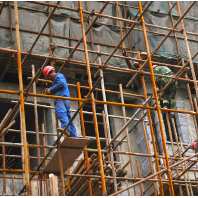
\includegraphics[width=0.6\textwidth]{./chapters/cap3}
\end{figure}

%%%%%%%%%%%%%%%%%%%%%%%%%%%%%%%%%%%%%%%%%%%
%%%%%%  STYLE 32
%%%%%%%%%%%%%%%%%%%%%%%%%%%%%%%%%%%%%%%%%%%

\cxset{
 name={},
 numbering=arabic,
 number font-size=\HUGE,
 number font-family=\sffamily,
 number font-weight=\bfseries,
 number before={\hspace*{-20pt}},
 number position=leftname,
 chapter font-family=\sffamily,
 chapter font-weight=\normalfont,
 chapter font-size=\small,
 number after={},
 chapter before={\vspace*{50pt}\par\hspace*{-50pt}},
 chapter after={\hspace*{20pt}},
 chapter color={black!90},
 number color=\color{black!90},
 title beforeskip={},
 title afterskip={\vspace{50pt}},
 title before=,
 title after={\par},
 title font-family=\itshape,
 title font-color=\color{black!80},
 title font-weight=\itshape,
 title font-size=\LARGE}
\chapter{Introduction to Style Thirty Two}

This style has a modern look to it. Its main characteristic is the large chapter number and the fact that it is drawn into the margin. A common style for computer books.
\medskip
\begin{figure}[ht]
\centering
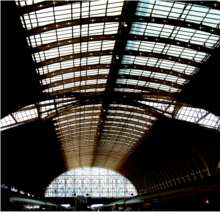
\includegraphics[width=0.6\textwidth]{./chapters/cap3a}
\end{figure}
The example is from Python NLP book.

%%%%%%%%%%%%%%%%%%%%%%%%%%%%%%%%%%%%%%%%%%%
%%%%%%  STYLE 33
%%%%%%%%%%%%%%%%%%%%%%%%%%%%%%%%%%%%%%%%%%%

\cxset{
 name=CHAPTER,
 numbering=Roman,
 number font-size=\small,
 number font-family=\rmfamily,
 number font-weight=\normalfont,
 number before={},
 number position=rightname,
 chapter font-family=\sffamily,
 chapter font-weight=\normalfont,
 chapter font-size=\small,
 number after={},
 chapter before={},
 chapter after={\par},
 chapter color={black!90},
 number color=\color{black!90},
 title beforeskip={},
 title afterskip={\vspace{50pt}},
 title before=,
 title after={\par},
 title font-family=\normalfont,
 title font-color=\color{black!80},
 title font-weight=\normalfont,
 title font-size=\LARGE}
\chapter{Introduction to Style Thirty Three}

The interesting part of this style is that it uses roman numerals to display the counter that is in a different font than that used for the chapter name.
\medskip
\begin{figure}[ht]
\centering
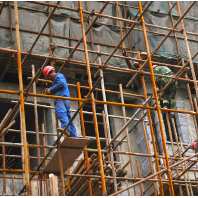
\includegraphics[width=0.6\textwidth]{./chapters/cap3}
\end{figure}





%%%%%%%%%%%%%%%%%%%%%%%%%%%%%%%%%%%%%%%%%%%
%%%%%%  STYLE 34
%%%%%%%%%%%%%%%%%%%%%%%%%%%%%%%%%%%%%%%%%%%

\cxset{
 name=CHAPTER,
 numbering=Roman,
 number font-size=\small,
 number font-family=\rmfamily,
 number font-weight=\normalfont,
 number before={},
 number position=rightname,
 chapter font-family=\sffamily,
 chapter font-weight=\normalfont,
 chapter font-size=\small,
 number after={},
 chapter before={},
 chapter after={\par},
 chapter color={black!90},
 number color=\color{black!90},
 title beforeskip={},
 title afterskip={\vspace{50pt}},
 title before=,
 title after={\par},
 title font-family=\normalfont,
 title font-color=\color{black!80},
 title font-weight=\normalfont,
 title font-size=\LARGE}
\section{Introduction to Style Thirty Four}

The interesting part of this style is that it uses roman numerals to display the counter that is in a different font than that used for the chapter name.
\medskip
\begin{figure}[ht]
\centering
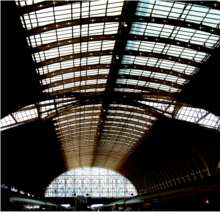
\includegraphics[width=0.6\textwidth]{./chapters/cap3a}
\end{figure}


%%%%%%%%%%%%%%%%%%%%%%%%%%%%%%%%%%%%%%%%%%%
%%%%%%  STYLE 35
%%%%%%%%%%%%%%%%%%%%%%%%%%%%%%%%%%%%%%%%%%%

\cxset{%
 name=CHAPTER,
 numbering=Roman,
 number font-size=\small,
 number font-family=\rmfamily,
 number font-weight=\normalfont,
 number before={},
 number position=rightname,
 chapter font-family=\sffamily,
 chapter font-weight=\normalfont,
 chapter font-size=\small,
 number after={},
 chapter before={},
 chapter after={\par},
 chapter color={black!90},
 number color=\color{black!90},
 title beforeskip={},
 title afterskip={\vspace{50pt}},
 title before=,
 title after={\par},
 title font-family=\normalfont,
 title font-color=\color{black!80},
 title font-weight=\normalfont,
 title font-size=\LARGE}
\chapter{Introduction to Style Thirty Five}

The interesting part of this style is that it uses roman numerals to display the counter that is in a different font than that used for the chapter name.
\medskip

\begin{figure}[ht]
\centering
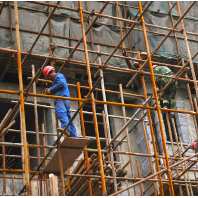
\includegraphics[width=0.6\textwidth]{./chapters/cap3}
\end{figure}


%%%%%%%%%%%%%%%%%%%%%%%%%%%%%%%%%%%%%%%%%%%
%%%%%%  STYLE 36
%%%%%%%%%%%%%%%%%%%%%%%%%%%%%%%%%%%%%%%%%%%

\cxset{
 name=CHAPTER,
 numbering=Roman,
 number font-size=\small,
 number font-family=\rmfamily,
 number font-weight=\normalfont,
 number before={},
 number position=rightname,
 chapter font-family=\sffamily,
 chapter font-weight=\normalfont,
 chapter font-size=\small,
 number after={},
 chapter before={},
 chapter after={\par},
 chapter color={black!90},
 number color=\color{black!90},
 title beforeskip={},
 title afterskip={\vspace{50pt}},
 title before=,
 title after={\par},
 title font-family=\normalfont,
 title font-color=\color{black!80},
 title font-weight=\normalfont,
 title font-size=\LARGE}
\chapter{Introduction to Style Thirty Six}

The interesting part of this style is that it uses roman numerals to display the counter that is in a different font than that used for the chapter name.
\medskip

\begin{figure}[ht]
\centering
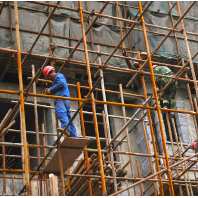
\includegraphics[width=0.6\textwidth]{./chapters/cap3}
\end{figure}


%%%%%%%%%%%%%%%%%%%%%%%%%%%%%%%%%%%%%%%%%%%
%%%%%%  STYLE 37
%%%%%%%%%%%%%%%%%%%%%%%%%%%%%%%%%%%%%%%%%%%

\cxset{
 name=CHAPTER,
 numbering=Roman,
 number font-size=\small,
 number font-family=\rmfamily,
 number font-weight=\normalfont,
 number before={},
 number position=rightname,
 chapter font-family=\sffamily,
 chapter font-weight=\normalfont,
 chapter font-size=\small,
 number after={},
 chapter before={},
 chapter after={\par},
 chapter color={black!90},
 number color=\color{black!90},
 title beforeskip={},
 title afterskip={\vspace{50pt}},
 title before=,
 title after={\par},
 title font-family=\normalfont,
 title font-color=\color{black!80},
 title font-weight=\normalfont,
 title font-size=\LARGE}
\chapter{Introduction to Style Thirty Seven}

The interesting part of this style is that it uses roman numerals to display the counter that is in a different font than that used for the chapter name.
\medskip

\begin{figure}[ht]
\centering
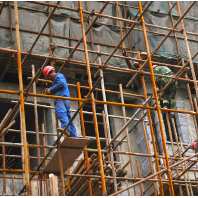
\includegraphics[width=0.6\textwidth]{./chapters/cap3}
\end{figure}


%%%%%%%%%%%%%%%%%%%%%%%%%%%%%%%%%%%%%%%%%%%
%%%%%%  STYLE 38
%%%%%%%%%%%%%%%%%%%%%%%%%%%%%%%%%%%%%%%%%%%

\cxset{
 name=CHAPTER,
 numbering=arabic,
 number font-size=\LARGE,
 number font-family=\sffamily,
 number font-weight=\bfseries,
 number before={},
 number position=rightname,
 chapter font-family=\sffamily,
 chapter font-weight=\bfseries,
 number after={},
 chapter before={\rule{\textwidth}{2pt}\par},
 chapter after={\vskip0pt\vspace*{-8pt}\rule{\textwidth}{.4pt}\vskip-7pt},
 chapter color={black!90},
 number color=\color{black!90},
 title beforeskip={},
 title afterskip={\vspace{50pt}},
 title before=,
 title after={\par\vskip-19pt\rule{\textwidth}{0.4pt}\par} ,
 title font-family=\sffamily,
 title font-color=\color{black!80},
 title font-weight=\bfseries,
 title font-size=\LARGE,
 chapter font-size=\LARGE}
\chapter{INTRODUCTION}

This style uses rules to enclose both the chapter name and number as well as the title, which necessarily needs to be rather short.
\medskip

\begin{figure}[ht]
\centering
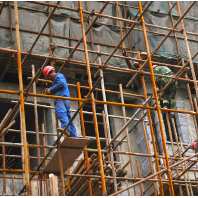
\includegraphics[width=0.6\textwidth]{./chapters/cap3}
\end{figure}



%%%%%%%%%%%%%%%%%%%%%%%%%%%%%%%%%%%%%%%%%%%
%%%%%%  STYLE 39
%%%%%%%%%%%%%%%%%%%%%%%%%%%%%%%%%%%%%%%%%%%

\cxset{
 name=CHAPTER,
 numbering=arabic,
 number font-size=\LARGE,
 number font-family=\sffamily,
 number font-weight=\bfseries,
 number before={},
 number position=rightname,
 chapter font-family=\sffamily,
 chapter font-weight=\bfseries,
 number after={},
 chapter before={\rule{\textwidth}{2pt}\par},
 chapter after={\vskip0pt\vspace*{-8pt}\rule{\textwidth}{.4pt}\vskip-7pt},
 chapter color={black!90},
 number color=\color{black!90},
 title beforeskip={},
 title afterskip={\vspace{50pt}},
 title before=,
 title after={\par\vskip-19pt\rule{\textwidth}{0.4pt}\par} ,
 title font-family=\sffamily,
 title font-color=\color{black!80},
 title font-weight=\bfseries,
 title font-size=\LARGE,
 chapter font-size=\LARGE}
\chapter{INTRODUCTION}

This style uses rules to enclose both the chapter name and number as well as the title, which necessarily needs to be rather short.
\medskip

\begin{figure}[ht]
\centering
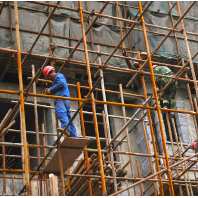
\includegraphics[width=0.6\textwidth]{./chapters/cap3}
\end{figure}
In the picture it does not look very attractive, but in the actual book it does. My observation is that the rule clearances are a bit tight and if you use this type of layout it is better to experiment until you get them right.

\begin{tcblisting}{}
\@makechapterhead[
 name=CHAPTER,
 numbering=arabic,
 number font-size=\LARGE,
 number font-family=\sffamily,
 number font-weight=\bfseries,
 number before={},
 number position=rightname,
 chapter font-family=\sffamily,
 chapter font-weight=\bfseries,
 number after={},
 chapter before={\rule{\textwidth}{2pt}\par},
 chapter after={\vskip0pt\vspace*{-8pt}\rule{\textwidth}{.4pt}\vskip-7pt},
 chapter color={black!90},
 number color=\color{black!90},
 title beforeskip={},
 title afterskip={\vspace{50pt}},
 title before=,
 title after={\par\vskip-19pt\rule{\textwidth}{0.4pt}\par} ,
 title font-family=\sffamily,
 title font-color=\color{black!80},
 title font-weight=\bfseries,
 title font-size=\LARGE,
 chapter font-size=\LARGE]{INTRODUCTION}
\end{tcblisting}


%%%%%%%%%%%%%%%%%%%%%%%%%%%%%%%%%%%%%%%%%%%
%%%%%%  STYLE 40
%%%%%%%%%%%%%%%%%%%%%%%%%%%%%%%%%%%%%%%%%%%

\cxset{
 name=,
 numbering=arabic,
 number font-size=\LARGE,
 number font-family=\sffamily,
 number font-weight=\bfseries,
 number before={},
 number position=rightname,
 chapter font-family=\sffamily,
 chapter font-weight=\bfseries,
 chapter before=\hfill,
 number after=,
 chapter after=\hfill\hfill\vskip0pt ,
 chapter color={black!90},
 number color=\color{black!90},
 title beforeskip=,
 title before=\begin{center},
 title after=\end{center},
 title font-family=\sffamily,
 title font-color=\color{black!80},
 title font-weight=\bfseries,
 title font-size=\LARGE,
 chapter font-size=\LARGE}
\chapter{Introduction:\\ On Why and How How to Use\\ Chapter Style Forty}

A classical style chapter style with finely spaced out letters. A number of books spell out the chapter numbers. In general I find this as a good idea as sometimes the numbers don't blend in very well.

\begin{figure}[ht]
\centering
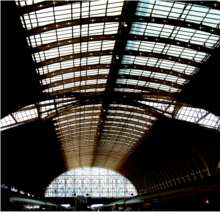
\includegraphics[width=0.6\textwidth]{./chapters/cap3a}
\end{figure}







%%%%%%%%%%%%%%%%%%%%%%%%%%%%%%%%%%%%%%%%%%%
%%%%%%  STYLE 41
%%%%%%%%%%%%%%%%%%%%%%%%%%%%%%%%%%%%%%%%%%%

\cxset{
 color=purple,
 name=CHAPTER,
 numbering=arabic,
 number font-size=\large,
 number font-family=\rmfamily,
 number font-weight=\normalfont,
 number before={},
 number position=rightname,
 chapter font-family=\rmfamily,
 chapter font-weight=\normalfont,
 chapter before=\hfill,
 number after=,
 chapter after=\hfill\hfill\vskip0pt ,
 chapter color={black!90},
 number color=\color{black!90},
 title beforeskip=,
 title before=\begin{center},
 title after=\end{center},
 title font-family=\rmfamily,
 title font-color=\color{black!80},
 title font-weight=\normalfont,
 title font-size=\LARGE,
 chapter font-size=\large}
\chapter{INTRODUCTION\\ TO CHAPTER STYLE FORTY ONE}
A classical style chapter style with finely spaced out letters. A number of books spell out the chapter numbers. In general I find this as a good idea as sometimes the numbers don't blend in very well.

\begin{figure}[ht]
\centering
\fbox{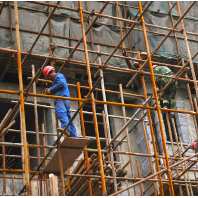
\includegraphics[width=0.6\textwidth]{./chapters/cap3}}
\end{figure}

 This book has different chapters written by different authors and the author's name appear below an ornament. don't dismiss ornaments as old fashioned as a lot of modern books still use them.



\cxset{
 name=,
 numbering=arabic,
 number font-size=\LARGE,
 number before={},
 number position=leftname,
 chapter before=\vspace*{10pt},
 number after=\hfill\hfill,
 chapter after=\hfill\hfill\vskip20pt ,
 number color=\color{gray},
 title font-family=\sffamily,
 title font-color=\color{black!80},
 title font-weight=,
 title font-size=\LARGE,
 chapter font-size=\huge}
\chapter{Introduction to Style 42}


Style 42 is shown in the following figure:

\begin{figure}[ht]
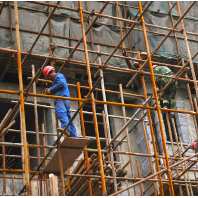
\includegraphics[width=0.6\textwidth]{./chapters/cap3}
\end{figure}
The distinguishing characteristics of this chapter are that it has an epigraph and is composed of very simple stylistic elements. The epigraph is placed quite a bit lower than the chapter title. The heading style is just the page number and underlined. 

%% Chapter 43 Style 43

\cxset{
 name=CHAPTER,
 numbering=arabic,
 number font-size=\Large,
 number before={},
 number position=rightname,
 chapter color={black!80},
 chapter font-size=\Large,
 chapter before=\par\hfill\hfill,
 number after=,
 chapter after=\vskip20pt ,
 number color=\color{black!80},
 title font-family=\itshape,
 title font-color=\color{black!80},
 title font-weight=,
 title font-size=\LARGE,
 title beforeskip=\hfill,header style=empty}
\chapter{Introduction to Style 43}


This style is reminiscent of the stylistic elements found in Tufte's books with the chapter title set in italics. 
\begin{figure}[ht]
\includegraphics[width=0.6\textwidth]{./chapters/cap3}
\end{figure}
I saw this style in the \textit{The Great Syrian Revolution and the Rise of Arab Nationalism} by Michael Provence, published by the University of Texas at Austin (2005). Notably the best part of the first page is taken by epigraphs. The chapter opens on an even page and bear no headers or footers. The large dropcap at the start of the chapter text balances the ragged left elements of the chapter block.

%% Style 45


\cxset{
 name=CHAPTER,
 numbering=arabic,
 number font-size=\Large,
 number before={},
 number position=rightname,
 chapter color={black!80},
 chapter font-size=\Large,
 chapter before=\par\hfill\hfill,
 number after=,
 chapter after=\vskip20pt ,
 number color=\color{black!80},
 title font-family=\itshape,
 title font-color=\color{black!80},
 title font-weight=,
 title font-size=\LARGE,
 title beforeskip=\hfill,header style=empty}
\chapter{Introduction to Style 45}


This is an unusual book with a rather unique style. The vertical rule is simple and breaks the monotony of a book that is heavy on text.
\begin{figure}[ht]
\includegraphics[width=0.6\textwidth]{./chapters/cap3a}
\end{figure}


UNITED ARAB EMIRATES
a new perspective
Edited by
IBRAHIM AL ABED
PETER HELLYERTrident Press Ltd
Layout and design,1997, 2001 Trident Press Ltd,UK.


%% Style 46

\cxset{,
 name=CHAPTER,
 numbering=arabic,
 number font-size=\Large,
 number before={},
 number position=rightname,
 chapter color={black!80},
 chapter font-size=\Large,
 chapter before=\par\hfill\hfill,
 number after=,
 chapter after=\vskip20pt ,
 number color=\color{black!80},
 title font-family=\itshape,
 title font-color=\color{black!80},
 title font-weight=,
 title font-size=\LARGE,
 title beforeskip=\hfill,header style=empty}
\section{Introduction to Style 46}


This is an unusual book with a rather unique style. The vertical rule is simple and breaks the monotony of a book that is heavy on text.
\begin{figure}[ht]
\includegraphics[width=0.45\textwidth]{./chapters/cap3}
\includegraphics[width=0.45\textwidth]{./chapters/cap3a}
\end{figure}

Understanding the Arab Culture a cross-cultural guide, second edition, published by How To Content, Dr Jehad Al-Omari,2008.

%% Style 48


\cxset{
 name=CHAPTER,
 numbering=arabic,
 number font-size=\Large,
 number before={},
 number position=rightname,
 chapter color={black!80},
 chapter font-size=\Large,
 chapter before=\par\hfill\hfill,
 number after=,
 chapter after=\vskip20pt ,
 number color=\color{black!80},
 title font-family=\itshape,
 title font-color=\color{black!80},
 title font-weight=,
 title font-size=\LARGE,
 title beforeskip=\hfill,
 header style=empty}
\chapter{Introduction to Style 46}


This is an unusual book with a rather unique style. The vertical rule is simple and breaks the monotony of a book that is heavy on text.
\begin{figure}[ht]
\includegraphics[width=0.48\textwidth]{./chapters/cap3}\hfill
\includegraphics[width=0.48\textwidth]{./chapters/cap3a}
\caption{Style 48 from the Oxford Handbook of Cuneiform Culture.}
\end{figure}

This style is very modern and typical of many computer books. The difficulty is in integrating all the page elements to make it work flawlessly.

The Oxford handbook of cuneiform Culture


%% Style 49

\cxset{
 name=CHAPTER,
 numbering=arabic,
 number font-size=\Large,
 number before={},
 number position=rightname,
 chapter color={black!80},
 chapter font-size=\Large,
 chapter before=\par\hfill\hfill,
 number after=,
 chapter after=\vskip20pt ,
 number color=\color{black!80},
 title font-family=\itshape,
 title font-color=\color{black!80},
 title font-weight=,
 title font-size=\LARGE,
 title beforeskip=\hfill,
 header style=empty}
\chapter{Introduction to Style 49}


This is an unusual book with a rather unique style. The vertical rule is simple and breaks the monotony of a book that is heavy on text.
\begin{figure}[ht]
\includegraphics[width=0.48\textwidth]{./chapters/cap3}\hfill
\includegraphics[width=0.48\textwidth]{./chapters/cap3a}
\caption{Style 48 from the Oxford Handbook of Cuneiform Culture.}
\end{figure}

This style is very modern and typical of many computer books. The difficulty is in integrating all the page elements to make it work flawlessly.

The Twenty-four
Hour Mind
The Role of Sleep and Dreaming in
Our Emotional Lives
Rosalind D. Cartwright



%% Style 50

\cxset{
 name=CHAPTER,
 numbering=arabic,
 number font-size=\Large,
 number before={},
 number position=rightname,
 chapter color={black!80},
 chapter font-size=\Large,
 chapter before=\par\hfill\hfill,
 number after=,
 chapter after=\vskip20pt ,
 number color=\color{black!80},
 title font-family=\itshape,
 title font-color=\color{black!80},
 title font-weight=,
 title font-size=\LARGE,
 title beforeskip=\hfill,
 header style=empty}
 \chapter{Introduction to Style 50}


This is an unusual book with a rather unique style. The vertical rule is simple and breaks the monotony of a book that is heavy on text.
\begin{figure}[ht]
\includegraphics[width=0.48\textwidth]{./chapters/cap3}\hfill
\includegraphics[width=0.48\textwidth]{./chapters/cap3a}
\caption{Style 50 from the Oxford Handbook of Cuneiform Culture.}
\end{figure}

This style is very modern and typical of many computer books. The difficulty is in integrating all the page elements to make it work flawlessly.

The psychology of facial
expression
Edited by
James A. Russell
University of British Columbia
Jose Miguel Fernandez-Dols
Universidad Autonoma de Madrid, Cambridge University Press.

%% Style 51

\cxset{
 name=CHAPTER,
 numbering=arabic,
 number font-size=\Large,
 number before={},
 number position=rightname,
 chapter color={black!80},
 chapter font-size=\Large,
 chapter before=\par\hfill\hfill,
 number after=,
 chapter after=\vskip20pt ,
 number color=\color{black!80},
 title font-family=\itshape,
 title font-color=\color{black!80},
 title font-weight=,
 title font-size=\LARGE,
 title beforeskip=\hfill,
 header style=empty}
\chapter{Introduction to Style 51}


This is an unusual book with a rather unique style. The vertical rule is simple and breaks the monotony of a book that is heavy on text.
\begin{figure}[ht]
\includegraphics[width=0.48\textwidth]{./chapters/cap3}\hfill
\includegraphics[width=0.48\textwidth]{./chapters/cap3a}
\caption{Style 50 from the Oxford Handbook of Cuneiform Culture.}
\end{figure}

This style is very modern and typical of many computer books. The difficulty is in integrating all the page elements to make it work flawlessly.

The psychology of facial
expression
Edited by
James A. Russell
University of British Columbia
Jose Miguel Fernandez-Dols
Universidad Autonoma de Madrid, Cambridge University Press.

%% Style 52


\cxset{
 name=CHAPTER,
 numbering=arabic,
 number font-size=\large,
 number before={},
 number position=rightname,
 chapter color={black!80},
 chapter font-size=\large,
 chapter before=\rule[3pt]{\textwidth}{0.4pt}\par\hfill,
 number after=,
 chapter after=\hfill\hfill\par\rule[6pt]{\textwidth}{0.4pt}\par,
 number color=\color{black!80},
 title font-family=\bfseries,
 title font-color=\color{black!80},
 title font-weight=,
 title font-size=\LARGE,
 title beforeskip=\hfill\par\hspace*{0pt},
 header style=empty}

\chapter{Introduction to Style Fifty Two}


This is an unusual book with a rather unique style. The vertical rule is simple and breaks the monotony of a book that is heavy on text.
\begin{figure}[ht]
\includegraphics[width=0.48\textwidth]{./chapters/cap3}\hfill
\includegraphics[width=0.48\textwidth]{./chapters/cap3a}
\caption{Style 50 from the Oxford Handbook of Cuneiform Culture.}
\end{figure}

This style is very modern and typical of many computer books. The difficulty is in integrating all the page elements to make it work flawlessly.

THE
LINGUISTICS
WARS, RANDY ALLEN HARRIS

%% Style 53


\cxset{
 name=,
 numbering=arabic,
 number font-size=\Large,
 number before={},
 number after=,
 number dot=,
 number position=rightname,
 number color=\color{blue},
 chapter color={blue},
 chapter font-size=\Large,
 chapter before=\par\hfill\hfill,
 chapter after=\hfill,
 title font-family=\rmfamily,
 title font-color=\color{blue},
 title font-weight=,
 title font-size=\LARGE,
 title beforeskip=\hfill,
 title afterskip=\leavevmode\center\rule{3cm}{0.4pt}\vskip-17pt\rule{3cm}{0.4pt}\endcenter\vskip10pt,
 header style=empty}
\chapter{\so{STYLE FIFTY THREE}}


This is an unusual book with a rather unique style. The vertical rule is simple and breaks the monotony of a book that is heavy on text.
\begin{figure}[ht]
\includegraphics[width=0.48\textwidth]{./chapters/cap3}\hfill
\includegraphics[width=0.48\textwidth]{./chapters/cap3a}
\caption{Style 50 from the Oxford Handbook of Cuneiform Culture.}
\end{figure}

T h e
JESUS
FAMILY
TOMB
The Discovery, the Investigation,
and the Evidence
That Could Change History
SIMCHA JACOBOVICI and CHARLES PELLEGRINO

Harper Collins 



%% Style 54

\cxset{
 name=,
 numbering=arabic,
 number font-size=\Large,
 number before={},
 number after=,
 number dot=,
 number position=rightname,
 number color=\color{blue},
 chapter color={blue},
 chapter font-size=\Large,
 chapter before=\par\hfill\hfill,
 chapter after=\hfill,
 title font-family=\rmfamily,
 title font-color=\color{blue},
 title font-weight=,
 title font-size=\LARGE,
 title beforeskip=\hfill,
 title afterskip={\vspace*{20pt}},
 header style=empty}
\chapter{\so{STYLE FIFTY FOUR}}


This is an unusual book with a rather unique style. The vertical rule is simple and breaks the monotony of a book that is heavy on text.\index{rules!style 54}

\begin{figure}[ht]
\fbox{\includegraphics[width=0.48\textwidth]{./chapters/cap3}}\hfill
\fbox{\includegraphics[width=0.48\textwidth]{./chapters/cap3a}}
\caption{Style 50 from the Oxford Handbook of Cuneiform Culture.}
\end{figure}

\end{document}
https://docs.google.com/open?id=0B75n0wtctw00RDhYSkIwOTBRRHU5Rl93Q19lalRlQQ